% This is "sig-alternate.tex" V2.0 May 2012
% This file should be compiled with V2.5 of "sig-alternate.cls" May 2012
%
% This example file demonstrates the use of the 'sig-alternate.cls'
% V2.5 LaTeX2e document class file. It is for those submitting
% articles to ACM Conference Proceedings WHO DO NOT WISH TO
% STRICTLY ADHERE TO THE SIGS (PUBS-BOARD-ENDORSED) STYLE.
% The 'sig-alternate.cls' file will produce a similar-looking,
% albeit, 'tighter' paper resulting in, invariably, fewer pages.
%
% ------------------------------------------------------------------------------
% This .tex file (and associated .cls V2.5) produces:
%       1) The Permission Statement
%       2) The Conference (location) Info information
%       3) The Copyright Line with ACM data
%       4) NO page numbers
%
% as against the acm_proc_article-sp.cls file which
% DOES NOT produce 1) thru' 3) above.
%
% Using 'sig-alternate.cls' you have control, however, from within
% the source .tex file, over both the CopyrightYear
% (defaulted to 200X) and the ACM Copyright Data
% (defaulted to X-XXXXX-XX-X/XX/XX).
% e.g.
% \CopyrightYear{2007} will cause 2007 to appear in the copyright line.
% \crdata{0-12345-67-8/90/12} will cause 0-12345-67-8/90/12 to appear in the copyright line.
%
% ------------------------------------------------------------------------------
% This .tex source is an example which *does* use
% the .bib file (from which the .bbl file % is produced).
% REMEMBER HOWEVER: After having produced the .bbl file,
% and prior to final submission, you *NEED* to 'insert'
% your .bbl file into your source .tex file so as to provide
% ONE 'self-contained' source file.
%
% ================= IF YOU HAVE QUESTIONS =======================
% Questions regarding the SIGS styles, SIGS policies and
% procedures, Conferences etc. should be sent to
% Adrienne Griscti (griscti@acm.org)
%
% Technical questions _only_ to
% Gerald Murray (murray@hq.acm.org)
% ===============================================================
%
% For tracking purposes - this is V2.0 - May 2012


%\documentclass[preprint]{sig-alternate}
\documentclass{svmult}
\synctex=1
%\usepackage{srcltx}
\usepackage[T1]{fontenc}
\usepackage[utf8]{inputenc}
\usepackage{tikz}
\usepackage{amssymb}
\usepackage{hyperref}
\usepackage{array}
%\newcommand{\url}[1] { \texttt{#1}}

\begin{document}
%
% --- Author Metadata here ---
%\conferenceinfo{IWOCL}{'15 Stanford}
%\CopyrightYear{2007} % Allows default copyright year (20XX) to be over-ridden - IF NEED BE.
%\crdata{0-12345-67-8/90/01}  % Allows default copyright data (0-89791-88-6/97/05) to be over-ridden - IF NEED BE.
% --- End of Author Metadata ---

\title*{Asynchronous OpenCL/MPI numerical simulations of conservation laws}
%\subtitle{[Extended Abstract]
%\titlenote{A full version of this paper is available as
%\textit{Author's Guide to Preparing ACM SIG Proceedings Using
%\LaTeX$2_\epsilon$\ and BibTeX} at
%\texttt{www.acm.org/eaddress.htm}}}
%
% You need the command \numberofauthors to handle the 'placement
% and alignment' of the authors beneath the title.
%
% For aesthetic reasons, we recommend 'three authors at a time'
% i.e. three 'name/affiliation blocks' be placed beneath the title.
%
% NOTE: You are NOT restricted in how many 'rows' of
% "name/affiliations" may appear. We just ask that you restrict
% the number of 'columns' to three.
%
% Because of the available 'opening page real-estate'
% we ask you to refrain from putting more than six authors
% (two rows with three columns) beneath the article title.
% More than six makes the first-page appear very cluttered indeed.
%
% Use the \alignauthor commands to handle the names
% and affiliations for an 'aesthetic maximum' of six authors.
% Add names, affiliations, addresses for
% the seventh etc. author(s) as the argument for the
% \additionalauthors command.
% These 'additional authors' will be output/set for you
% without further effort on your part as the last section in
% the body of your article BEFORE References or any Appendices.
\author{Philippe Helluy, Thomas Strub, Michel Massaro, Malcolm Roberts}

\institute{Philippe Helluy \at IRMA, Université de Strasbourg and Inria Tonus, France \email{helluy@unistra.fr}
\and Thomas Strub \at AxesSim Illkirch, France \email{thomas.strub@axessim.fr} 
\and Michel Massaro \at IRMA, Université de Strasbourg, France \email{massaro@math.unistra.fr}
\and Malcolm Roberts \at IRMA, Université de Strasbourg, France \email{roberts@math.unistra.fr} }
%\numberofauthors{4} %  in this sample file, there are a *total*
% of EIGHT authors. SIX appear on the 'first-page' (for formatting
% reasons) and the remaining two appear in the \additionalauthors section.
%
%\author{
%% You can go ahead and credit any number of authors here,
%% e.g. one 'row of three' or two rows (consisting of one row of three
%% and a second row of one, two or three).
%%
%% The command \alignauthor (no curly braces needed) should
%% precede each author name, affiliation/snail-mail address and
%% e-mail address. Additionally, tag each line of
%% affiliation/address with \affaddr, and tag the
%% e-mail address with \email.
%%
%% 1st. author
%\alignauthor
%Philippe Helluy \\%\titlenote{Dr.~Trovato insisted his name be first.}\\
%       \affaddr{IRMA, Université de Strasbourg}\\
%       \affaddr{and Inria TONUS} \\
%       \affaddr{7 rue Descartes}\\
%       \affaddr{Strasbourg, France}\\
%       \email{philippe.helluy@unistra.fr}
%% 2nd. author
%\alignauthor
%Thomas Strub\\
%%\titlenote{The secretary disavows
%%any knowledge of this author's actions.}\\
%       \affaddr{AxesSim}\\
%       \affaddr{rue Jean Sapidus}\\
%       \affaddr{Illkirch, France}\\
%       \email{thomas.strub@axessim.fr}
%% 3rd. author
%\alignauthor
%Michel Massaro\\
%%\titlenote{The secretary disavows
%%any knowledge of this author's actions.}\\
%       \affaddr{IRMA, Université de Strasbourg}\\
%       \affaddr{7 rue Descartes}\\
%       \affaddr{Strasbourg, France}\\
%       \email{michel.massaro@unistra.fr}
%% 3rd. author
%\and
%\alignauthor
%Malcolm Roberts\\
%%\titlenote{The secretary disavows
%%any knowledge of this author's actions.}\\
%       \affaddr{IRMA, Université de Strasbourg}\\
%       \affaddr{7 rue Descartes}\\
%       \affaddr{Strasbourg, France}\\
%       \email{malcolm.roberts@unistra.fr}
%}
%% There's nothing stopping you putting the seventh, eighth, etc.
%% author on the opening page (as the 'third row') but we ask,
%% for aesthetic reasons that you place these 'additional authors'
%% in the \additional authors block, viz.
%%\additionalauthors{Additional authors: John Smith (The Th{\o}rv{\"a}ld Group,
%%email: {\texttt{jsmith@affiliation.org}}) and Julius P.~Kumquat
%%(The Kumquat Consortium, email: {\texttt{jpkumquat@consortium.net}}).}
%\date{13 February 2015}
%% Just remember to make sure that the TOTAL number of authors
%% is the number that will appear on the first page PLUS the
%% number that will appear in the \additionalauthors section.
%
%\toappear{This work has benefited from several supports: from the French Defense Agency DGA, from the Labex ANR-11-LABX-0055-IRMIA and from the AxesSim company.}
\newcommand\open[2]{\ensuremath{]#1,#2[}}


\maketitle

\abstract{ Hyperbolic conservation laws are important mathematical
  models for describing many phenomena in physics or engineering.  The
  Finite Volume (FV) method and the Discontinuous Galerkin (DG)
  methods are two popular methods for solving conservation laws on
  computers.  In this paper, we present several FV and DG numerical
  simulations that we have realized with the OpenCL and MPI paradigms.
  First, we compare two optimized implementations of the FV method on
  a regular grid: an OpenCL implementation and a more traditional
  OpenMP implementation. We compare the efficiency of the approach on
  several CPU and GPU architectures of different brands.  Then we
  present how we have implemented the DG method in the OpenCL/MPI
  framework in order to achieve high efficiency. The implementation
  relies on a splitting of the DG mesh into sub-domains and
  sub-zones. Different kernels are compiled according to the zone
  properties. In addition, we rely on the OpenCL asynchronous task
  graph in order to overlap OpenCL computations, memory transfers and
  MPI communications.}

% A category with the (minimum) three required fields
%\category{H.4}{Information Systems Applications}{Miscellaneous}
%A category including the fourth, optional field follows...
%\category{D.2.8}{Software Engineering}{Metrics}[complexity measures, performance measures]

%\terms{Theory}

\keywords{OpenCL, MPI, task graph, conservation laws, discontinuous
  Galerkin approximation}

\section{Introduction}
Hyperbolic conservation laws are a particular class of Partial
Differential Equations (PDE) models. They are present in many fields
of physics or engineering. It is thus very important to have efficient
software tools for solving such systems.  The unknown of a system of
conservation laws is a vector $\vec{W}(\vec{x},t)\in \mathbb{R}^m$
that depends on a space variable $\vec{x}=(x^1,\ldots, x^d)$ and time
$t$. The vector $\vec{W}$ is called the vector of conservative
variables. In this work we shall consider a space dimension $d=2$ or
$d=3$. Generally, the space variable $\vec{x}$ belongs to a bounded
domain $\Omega\subset \mathbb{R}^d$. The system of conservation reads
\begin{equation}
  \partial_t \vec{W} + \partial_k \vec{F}^k(\vec{W})=0. \label{eq:conslaw}
\end{equation}
In this formula, we use the following notations:
\begin{itemize}
\item The partial derivative operators are denoted
  by \begin{equation}\partial_t = \frac{\partial}{\partial_t},\quad
    \partial_k = \frac{\partial}{\partial {x^k}}.\end{equation}
\item We adopt the Einstein sum-on-repeated-indices
  convention \begin{equation}\partial_k \vec{F}^k(\vec{W})
    =\sum_{k=1}^{d}\partial_k \vec{F}^k(\vec{W}).\end{equation}
\item The functions $\vec{F}^k(\vec{W})\in \mathbb{R}^m$, $k=1\ldots
  d$, characterize the physical model that we wish to represent. It is
  classic to consider a space vector $\vec{n}=(n_1\ldots
  n_d)\in\mathbb{R}^d$ and to also define the \textit{flux} of the
  system
  \begin{equation}
    \vec{F}(\vec{W},\vec{n})=\vec{F}^k(\vec{W})n_k.
  \end{equation}
\end{itemize}
System (\ref{eq:conslaw}) is supplemented by an initial condition
\begin{equation}\label{eq:init_cond}
  \vec{W}(\vec{x},0)=\vec{W}_0(\vec{x}),
\end{equation}
at time $t=0$, and conditions on the boundary $\partial \Omega$ of
$\Omega$. For example, one can prescribe the value of $\vec{W}$ on the
boundary
\begin{equation}\label{eq:boundary_cond}
\vec{W}(\vec{x},t)=\vec{W}_b(\vec{x},t),\quad \vec{x}\in\partial \Omega.
\end{equation}
Generally, the system (\ref{eq:conslaw}), (\ref{eq:init_cond}),
(\ref{eq:boundary_cond}) admits a unique solution if it satisfies the
hyperbolicity condition: the Jacobian matrix of the
flux \begin{equation}\nabla_{\vec{W}}
  \vec{F}(\vec{W},\vec{n})\end{equation} is diagonalizable with real
eigenvalues for all values of $\vec{W}$ and $\vec{n}$.

The above mathematical framework is very general. It can be applied to
electromagnetism, fluid mechanics, multiphase flows,
magneto-hydro-dynamics (MHD), Vlasov plasmas, \emph{etc}. Let us just
give two examples:
\begin{enumerate}
\item The Maxwell equations describe the evolution of the electric
  field $\vec{E}(\vec{x},t)\in \mathbb{R}^3$ and the magnetic field
  $\vec{H}(\vec{x},t)\in \mathbb{R}^3$. The conservative variables are
  the superimposition of these two vectors
  $\vec{W}=(\vec{E}^T,\vec{H}^T)^T$ (thus $m=6$) and the Maxwell flux
  is given
  by
  \begin{equation}\vec{F}(\vec{W},\vec{n})=\left[\begin{array}{cc}
        0 & -\vec{n}\times\\ \vec{n}\times & 0
      \end{array}\right]\vec{W}.
  \end{equation}
  In Sect.3 we present numerical results obtained with the Maxwell
  equations.
\item In fluid mechanics, the Euler equations describe the evolution
  of a compressible gas of density $\rho$, velocity
  $\vec{u}=(u^1,u^2,u^3)^T$ and pressure $p$. The conservative
  variables are given here by \begin{equation}W=(\rho,\rho
    \vec{u}^T,p/(\gamma-1)+1/2 \rho \vec{u}\cdot
    \vec{u})^T\end{equation} and the flux by \begin{equation}
      \vec{F}(\vec{W},\vec{n})=(\rho \vec{u} \cdot \vec{n}, \rho
      \vec{u}\cdot \vec{n} \vec{u}^T
      + \end{equation} \begin{equation}p \vec{n}^T,\left\{ \gamma
      p/(\gamma-1)+1/2 \rho \vec{u}\cdot \vec{u} \right\} \vec{u}\cdot
      \vec{n})^T,\end{equation}where $\gamma>1$ is the polytropic
    exponent of the gas. The MHD equations are a generalization of the
    Euler equations for taking into account magnetic effects in
    conductive compressible gas. The MHD system is a complicated
    system of conservation laws, with $m=9$. It is not the objective
    of this work to detail the MHD equations. For this we refer for
    instance to \cite{massaro2014numerical}. In Sect.2, we present
    numerical results obtained with the MHD equations.
\end{enumerate}

Because of their numerous fields of application, many numerical
methods have been developed for the resolution of hyperbolic
conservation laws. For instance the finite volume (FV) and
discontinuous Galerkin (DG) method are very popular. They are easy to
program on a standard parallel computer thanks to subdomain
decomposition. However, on new hybrid architectures, the efficient
implementation of those methods is more complex. It appears that there
is possibility of optimizations. In this paper, we explore several
numerical experiments that we have made for solving conservation laws
with the FV and DG methods on hybrid computers. OpenCL and MPI
libraries are today available on a wide range of platform, making them
a good choice for our optimizations.  It is classic to rely on OpenCL
for local computations and on MPI for communications between
accelerators. In addition, in our work we will see that it is
interesting to also use the OpenCL asynchronous task graph in order to
overlap OpenCL computations, memory transfers and MPI communications.

In the first part of this paper, we compare a classic OpenMP
optimization of a FV solver to an OpenCL implementation. We show that
on a standard multicore CPU, we obtain comparable speedups between the
OpenMP and the OpenCL implementation. In addition, using several GPU
accelerators and MPI communications between them, we were able to make
computations that would be unattainable with more classic
architectures.

Our FV implementation is limited to regular grids. In the second part
of the paper, we thus describe an efficient implementation of the DG
algorithm on unstructured grids.  Our implementation relies on several
standard optimizations: local memory prefetching, exploitation of the
sparse nature of the tensor basis, and MPI subdomain
decomposition. Other optimizations are less common: idling work-item
for minimizing cache prefetching and asynchronous MPI/OpenCL
communication.

\section{\label{fv}Comparison of an OpenCL and an OpenMP Solver on a Regular Grid}

\subsection{FV Approximation of Conservation Laws}

The FV and DG method construct a discontinuous approximation of the
conservative variables $W$. In the case of the FV method, the
approximation is piecewise constant. In the case of the DG method, the
approximation is piecewise polynomial. It is therefore necessary to
extend the definition of the flux $\vec{F}(\vec{W},\vec{n})$ at a
discontinuity of the solution. We consider thus a spatial
discontinuity $\Sigma$ of $\vec{W}$. The discontinuity is oriented by
a normal vector $\vec{n}_{LR}$. We use the following convention: the
``left'' (L) of $\Sigma$ is on the side of
$-\vec{n}_{LR}=\vec{n}_{RL}$ and the ``right'' (R) is on the side of
$\vec{n}_{LR}$. We denote by $\vec{W}_L$ and $\vec{W}_R$ the values of
$\vec{W}$ on the two sides of $\Sigma$. The numerical flux is then a
function
\begin{equation}
  \vec{F}(\vec{W}_L,\vec{W}_R,\vec{n}_{LR}).
\end{equation}
A common choice is to take the Lax-Friedrichs flux (see for instance
\cite{leveque2002finite} and included references)
\begin{equation}
  \vec{F}(\vec{W}_L,\vec{W}_R,\vec{n})
  =\frac{\vec{F}(\vec{W}_L,\vec{n})
    +\vec{F}(\vec{W}_R,\vec{n})}{2}-\frac{s}{2}(\vec{W}_R-\vec{W}_L),
\end{equation}
where $s$ is called the numerical viscosity. It is a supremum of all
the wave speeds of the system.  For more simplicity, in this section
we consider the two-dimensional case $d=2$ and a square domain
$\vec{x}=(x^1,x^2)\in \Omega=\open{0}{L}\times\open{0}{L}$. The space
step of the grid is $\Delta x=L/N$ where $N$ is a positive
integer. The grid cells are squares of size $h\times h$. The cell
centers are defined by $\vec{x}_{i,j}=((i+\frac{1}{2})\Delta
x,(j+\frac{1}{2})\Delta x)$. We also consider a time step $\Delta t$
and the times $t^n=n\Delta t$. We look for an approximation
$\vec{W}^n_{i,j}$ of $\vec{W}$ at the cell centers $\vec{x}_{i,j}$ and
at time $t^n$

\begin{equation}
  \vec{W}^n_{i,j}\simeq \vec{W}(\vec{x}_{i,j},t^n).
\end{equation}
Let $\vec{\nu}^1$ and $\vec{\nu}^2$ be normal vectors pointing in the
$x^1$ and $x^2$ direction, respectively, so that
\begin{equation}
  \vec{\nu}^1=(1,0)^T,\quad \vec{\nu}^2=(0,1)^T.
\end{equation}
We adopt a Strang dimensional splitting strategy: for advancing the
numerical solution from time step $t^n$ to time step $t^{n+1}$, we
first solve the finite volume approximation in direction $x^1$
\begin{equation}
  \frac{\vec{W}_{i,j}^{*}-\vec{W}_{i,j}^{n}}{\Delta t}+\frac{\vec{F}(\vec{W}^n_{i,j},\vec{W}^n_{i+1,j},\vec{\nu}^1)-\vec{F}(\vec{W}^n_{i-1,j},\vec{W}^n_{i,j},\vec{\nu}^1)}{\Delta x}=0,
\label{eq:x-step}
\end{equation}
and then in direction $x^2$
\begin{equation}
  \frac{\vec{W}_{i,j}^{n+1}-\vec{W}_{i,j}^{*}}{\Delta t}+\frac{\vec{F}(\vec{W}^n_{i,j},\vec{W}^n_{i,j+1},\vec{\nu}^2)-\vec{F}(\vec{W}^n_{i,j-1},\vec{W}^n_{i,j},\vec{\nu}^2)}{\Delta x}=0.
\label{eq:y-step}
\end{equation}
On the boundary cells, we simply replace, in the previous formulas,
the missing values of $\vec{W}$ by the boundary
values~(\ref{eq:boundary_cond}).

\subsection{OpenMP Implementation of the FV Scheme}
The chosen numerical scheme is very simple. We apply the FV scheme to
the ideal MHD system with divergence correction. The MHD system models
the coupling of a compressible fluid with a magnetic field. It
contains $m=9$ conservative variables and the numerical flux can be a
rather complex function. For more details and bibliography on the MHD
equations, we refer to \cite{massaro2014numerical}.

We have first written a C/OpenMP implementation of the algorithm. It
adopts a tiling strategy in order to avoid cache misses on large grids
with sizes bigger than 1024$\times$ 1024 points.  More details are
given in \cite{massaro2014numerical}. For later comparison with GPU
computations, we only consider results with single precision. We use
the optimized tiled OpenMP implementation as our reference for
comparisons with OpenCL implementations (see Table \ref{fv-speedup}
where the different implementations are compared).

\subsection{OpenCL Implementation of the FV Scheme}
\subsubsection{OpenCL}
It is necessary to adapt our code to new SIMD accelerators, such as
GPUs, in order to decrease computation cost. For this, we have chosen
OpenCL \cite{openclweb}, which is a programming framework, similar to
CUDA, for driving such accelerators. A feature of OpenCL is that
multicore CPUs are also considered as accelerators. The same program
can thus be run without modification on a CPU or a GPU.


\subsubsection{Implementation}
For the OpenCL version of our FV algorithm, we organize the data in a
$(x_{1},x_{2})$ grid: each conservative variable is stored in a
two-dimensional $(i,j)$ array. For advancing from time step $t^n$ to
time step $t^{n+1}$:
\begin{enumerate}
\item In principle, we associate an OpenCL thread (also called a
  work-item) to each cell of the grid and a thread block (also called
  a work-group) to each row. But OpenCL drivers generally impose a
  maximal work-group size. Thus when the row is too long it is also
  necessary to split the row and distribute it on several work-groups.
\item We compute the flux balance in the $x_{1}$-direction for each
  cell of each row of the grid (see formula (\ref{eq:x-step})).
\item We then transpose the grid, which amounts to exchanging the
  $x_{1}$ and $x_{2}$ coordinates. The $(i,j)\to (j,i)$ transposition
  is performed on the two-dimensional array of each conservative
  variable. For ensuring coalescent memory access we adopt an
  optimized memory transfer algorithm \cite{ruetsch2009optimizing}
  (see also \cite{michea2010accelerating}).
\item We can then compute the flux balance in the $x_{2}$-direction
  (\ref{eq:y-step}) for each row of the transposed grid. Because of
  the previous transposition, memory access is coalescent.
\item We again transpose the grid.
\end{enumerate}

Let us mention that other strategies are possible. For instance in
\cite{michea2010accelerating} the authors describe GPU computations of
scalar ($m=1$) elastic waves. The algorithm is based on
two-dimensional tiling of the mesh into cache memory and registers in
order to ensure fast memory access. However the tile size is limited
by the cache size and the number of unknowns $m$ in each grid cell. In
our case for the MHD system we have $m=9$ and the adaptation of the
algorithm given in \cite{michea2010accelerating} would probably be
inefficient.

We have tested this OpenCL implementation in several configurations.
See Table \ref{fv-speedup}. We can run the OpenCL code on a two-CPU
SMP computer or GPUs of different brands, without modification. In
addition, we obtain interesting speedups on SMP architectures. The
OpenCL speedup for CPU accelerator is approximately $70\%$ of the
OpenMP speedup. It remains very good considering that the
transposition algorithm probably deteriorates the memory access
efficiency on CPU architectures. The fact that OpenCL is a possible
alternative to OpenMP on multicore CPU has already been discussed in
\cite{shen2012performance}.

On AMD or NVIDIA GPUs, the same version of our code achieves good
performance. If we replace the optimized transposition by a naive
unoptimized transposition algorithm the code runs approximately 10
times slower on GPUs. The coalescent memory access is thus an
essential ingredient of the efficiency.

\subsection{OpenCL/MPI FV Solver}

We now modify the OpenCL implementation in order to address several
GPU accelerators at the same time. This could theoretically be
achieved by creating several command queues, one for each GPU
device. However, as of today, when GPUs are plugged into different
nodes of a supercomputer, the current OpenCL drivers are not able to
drive at the same time GPUs of different nodes. Therefore, we have
decided to rely on the MPI framework for managing the communications
between different GPUs. This strategy is very common (see for instance
\cite{aubert2010numerical,cabel2011multi,helluy2014two} and included
references).

We split the computational domain $\Omega$ into several subdomains in
the $x^1$ direction. An example of splitting with four subdomains is
presented on Fig.\ref{fig:mpi}.  Then, each subdomain is associated to
one MPI node and each MPI node drives one GPU. For applying the finite
volume algorithm on a subdomain, it is necessary to exchange two
layers of cells between the neighboring subdomains at the beginning of
each time step. The layers are shaded in grey in Fig.\ref{fig:mpi}. On
each MPI node, an exchange thus requires a GPU to CPU memory transfer
of the cell layers, a MPI send/recv communication and a CPU to GPU
transfer for retrieving the neighbor layers. The exchanged cells
represent a small amount of the total grid cells, however, the
transfer and communication time represent a non-negligible amount of
the computation cost.

In our first OpenCL/MPI implementation, the exchange task is performed
in a synchronous way: we wait for the exchange to be finished before
computing the flux balance in the subdomains.  This explains why the
speedup between the OpenCL code and the OpenCL/MPI code with four GPUs
is approximately 3.5 (the ideal speedup would be 4). See
Table~\ref{fv-speedup}).

Despite the synchronous approach, the OpenCL/MPI FV solver on
structured grid is rather efficient. It has permitted us to perform
computations on very fine grids that would be unreachable with
standard parallel computers. For instance, we have performed two-fluid
computations of shock-bubble interaction with grid size up to
$40,000\times 20,000$ in \cite{helluy2014interpolated}.

Now we would like to address the following drawbacks of the FV solver:
the FV method is limited to first or second order approximation; in
some applications, it is important to have access to higher order
schemes; MPI and host/GPU communications take time, so it is important
to provide asynchronous implementations for scalability with more MPI
nodes; finally, the previously described approach is limited to
structured grids and we wish also to extend the method to arbitrary
geometries.

In the next section we describe our implementation of a Discontinuous
Galerkin (DG) solver that allows to achieving higher order, addressing
general geometries, and overlapping computations and communications.
\begin{figure}
  \centering
  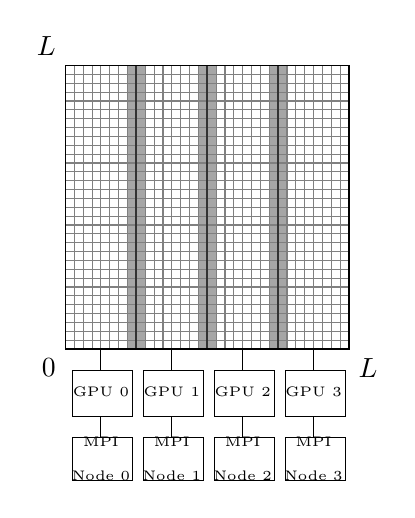
\begin{tikzpicture}[scale=0.9]
    \draw[color=gray] (0,0) grid[step=1./8] (4,4);
    \foreach \i in {1,2,3}{
      \draw[draw=gray, fill=gray!70] (-1./8+\i,0) grid[step=1./8] (1./8+\i,4) rectangle (-1./8+\i,0);
      \draw[color=black!80, thick] (\i,0) -- (\i,4);
    }
    \draw (0,0) rectangle (4,4);
    
    \foreach \i in {0,1,2,3}{
      \draw (\i+0.5,0) -- (\i+0.5,-0.3);
      \draw (\i+0.1,-0.95) rectangle (\i+0.95,-0.3);
      \node[align=center] at (\i+0.5,-0.6) {\tiny GPU \i};
      \draw (\i+0.5,-0.95) -- (\i+0.5,-1.25);
      \draw (\i+0.1,-1.85) rectangle (\i+0.95,-1.25);
      \node[align=center] at (\i+0.5,-1.55) {\tiny MPI\\\tiny Node \i};
    }

%\draw (0.5,-0.9) -- (0.5,-1.5) -- (1.2,-1.5);
%\draw (1.5,-0.9) -- (1.5,-1.2);
%\draw (2.5,-0.9) -- (2.5,-1.2);
%\draw (3.5,-0.9) -- (3.5,-1.5) -- (2.8,-1.5);
%\draw (1.2,-1.8) rectangle (2.8,-1.2);
%\node at (2,-1.5) {\tiny HOST};

    \node[below left] at (0,0) {$0$};
    \node[below right] at (4,0) {$L$};
    \node[above left] at (0,4) {$L$};
    
  \end{tikzpicture}
  \caption{Subdomain MPI decomposition\label{fig:mpi}}
\end{figure}

%\begin{figure}
%\centering
%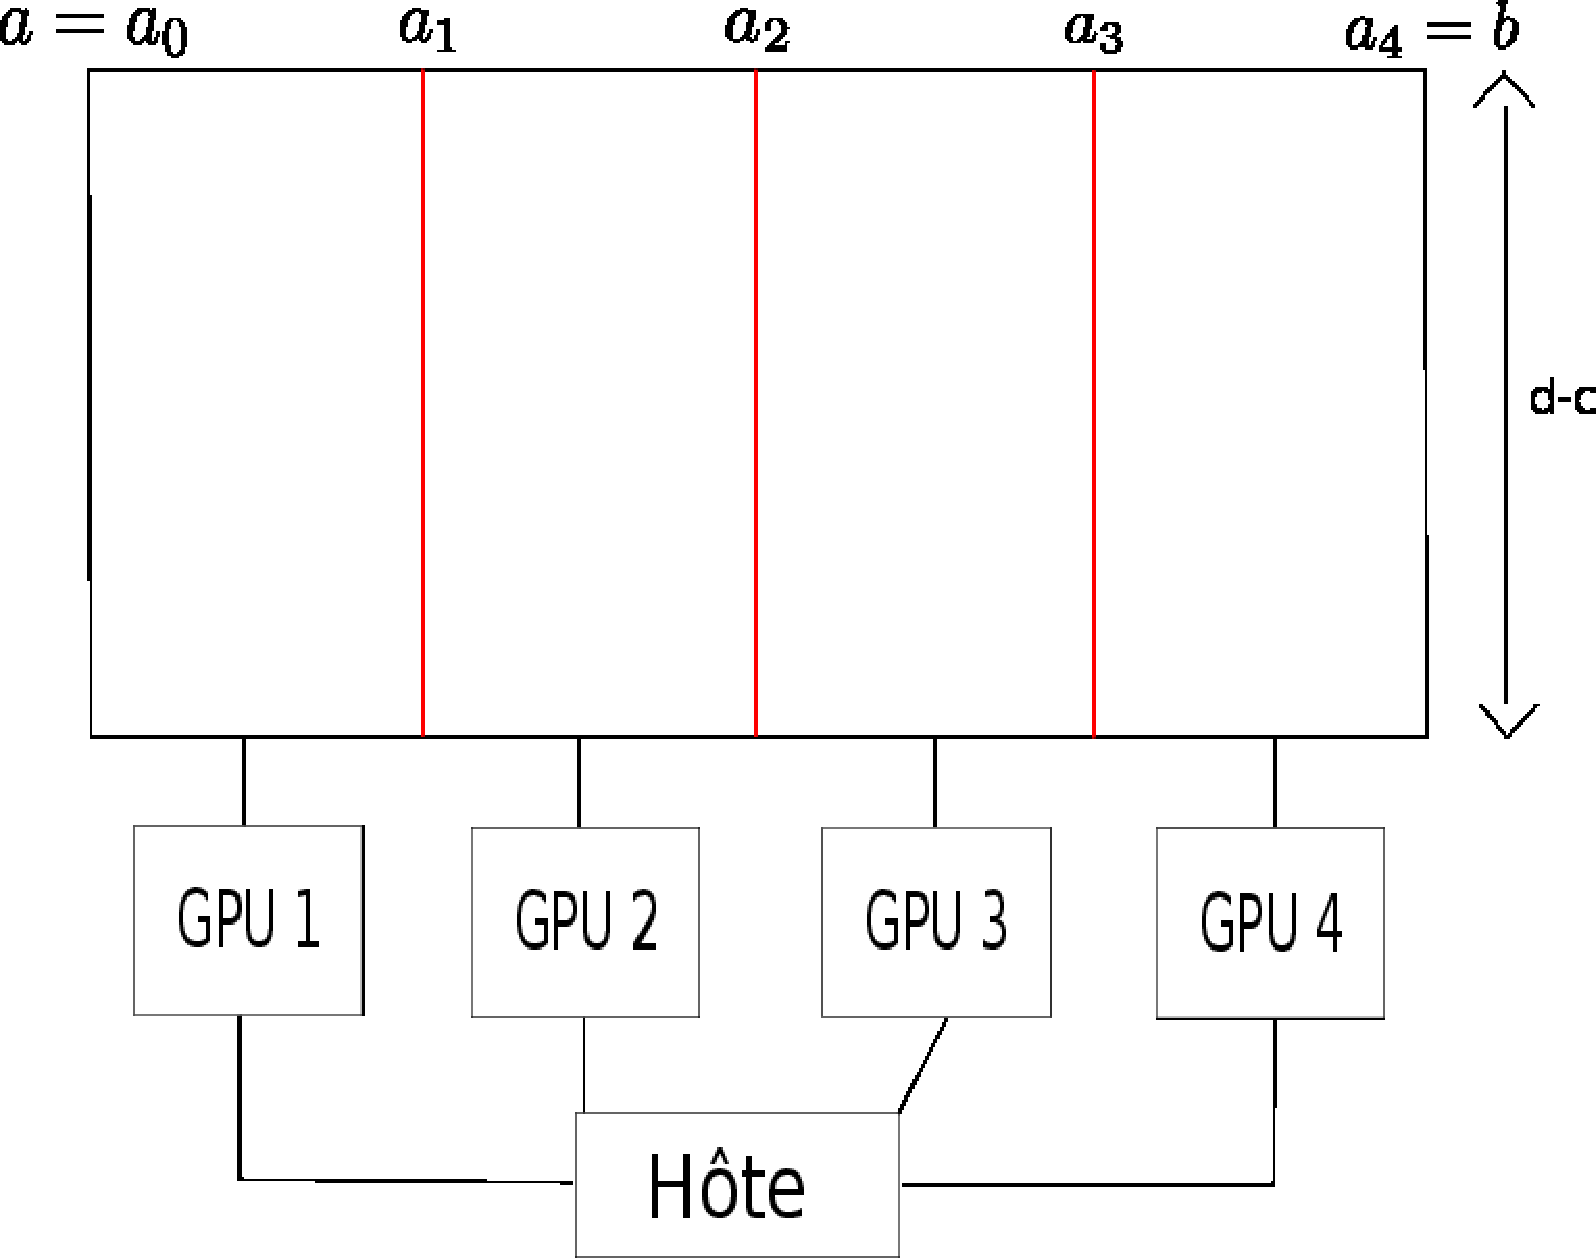
\includegraphics[width=6cm]{MPI.pdf}
%\caption{Subdomain MPI decomposition\label{fig:mpi}}
%\end{figure}

%\begin{figure}
%\centering
%\epsfig{file=fly.eps, height=1in, width=1in}
%\caption{A sample black and white graphic (.eps format)
%that has been resized with the \texttt{epsfig} command.}
%\end{figure}


%\begin{figure*}
%\centering
%\epsfig{file=flies.eps}
%\caption{A sample black and white graphic (.eps format)
%that needs to span two columns of text.}
%\end{figure*}


%
%\begin{table}
%\begin{tabular}{|c|c|c|}
%\hline
%Implementation & Time & Speedup\tabularnewline
%\hline
%\hline
%seq. code  & 30 days & 1\tabularnewline
%\hline
%seq. code -O3 & 146 h & 5\tabularnewline
%\hline
%seq. code -O3 + tiling & 97 h & 8\tabularnewline
%\hline
%OpenMP (Intel CPU 2x8 cores) & 6.2 h & 116\tabularnewline
%\hline
%OpenCL (Intel CPU 2x6 cores) & 18 h & 40\tabularnewline
%\hline
%OpenCL (NVIDIA K20) & 40 min & 1080\tabularnewline
%\hline
%OpenCL (AMD HD7970) & 32 min & 1325\tabularnewline
%\hline
%OpenCL + MPI (4 x NVIDIA K20) & 10 min & 3924\tabularnewline
%\hline
%\end{tabular}
%  \caption{Comparison of the different implementations of the FV scheme on a structured grid \label{fv-speedup}}
%
%\end{table}
%
%
%\begin{table}
%\begin{tabular}{|c|c|c|}
%\hline
%Implementation & Time & Speedup\tabularnewline
%\hline
%\hline
%OpenMP (Intel CPU 12 cores) & 863 s & 1\tabularnewline
%\hline
%OpenCL (Intel CPU 12 cores) & 2236 s & 0.3\tabularnewline
%\hline
%OpenCL (NVIDIA K20) & 60 s & 14\tabularnewline
%\hline
%OpenCL (AMD HD7970) & 49 s & 17\tabularnewline
%\hline
%OpenCL + MPI (4 x NVIDIA K20) & 17 s & 50\tabularnewline
%\hline
%\end{tabular}
% \caption{Comparison of the different implementations of the FV scheme on a
%   structured grid. Hardware : Intel(R) Xeon(R) E5-2630 (6 cores, 2.3GHz), AMD
%   Radeon 7950 (1792 cores, 2.8Gflops), NVidia K20m (2496 cores, 3.5 Gflops) \label{fv-speedup}}
%\end{table}
\begin{table}
  \centering
  \caption{Comparison of the different implementations of the FV scheme
    on a structured grid. Hardware : 2$\times$ Intel(R) Xeon(R) E5-2630
    (6 cores, 2.3GHz), AMD Radeon HD 7970, NVidia K20m. On Intel CPUs
    hyperthreading was deactivated \label{fv-speedup}}
  \begin{tabular}{|c|c|c|}
    \hline
    Implementation & Time & Speedup\tabularnewline
    \hline
    \hline
    OpenMP (Intel CPU 12 cores) & 717 s & 1\tabularnewline
    \hline
    OpenCL (Intel CPU 12 cores) & 996 s & 0.7\tabularnewline
    \hline
    OpenCL (NVIDIA K20) & 45 s & 16\tabularnewline
    \hline
    OpenCL (AMD HD7970) & 38 s & 19\tabularnewline
    \hline
    OpenCL + MPI (4 x NVIDIA K20) & 12 s & 58\tabularnewline
    \hline
  \end{tabular}

\end{table}


\section{\label{async}Asynchronous OpenCL/MPI Discontinuous Galerkin Solver}

We now present the Discontinuous Galerkin Method and explain our
software design for keeping high performance in the GPU
implementation.
\subsection{The DG Method}

\subsubsection{Interpolation on Unstructured Hexahedral Meshes}
The DG method is a generalization of the FV method. We suppose that
dimension $d=3$.  We consider a mesh of the computational domain
$\Omega$ made of cells $L_i$, $i=1\ldots N_c$.  In a cell $L$ of the
mesh, the field is approximated by a linear combination of basis
functions $\psi_j^L$
\begin{equation}\label{eq:expansion}
  \vec{W}(\vec{x},t)=\vec{W}_{L}^{j}(t)\psi_{j}^{L}(\vec{x}),\quad \vec{x}\in L.
\end{equation}

Each cell $L$ of the mesh is obtained by a geometrical mapping
$\tau_L$ that transforms a reference element $\hat L$ into $L$.  In
theory the shape of the reference element $\hat L$ may be arbitrary. A
classic choice is to consider tetrahedra \cite{hesthaven-2009}. In
this work we prefer hexahedra, as in \cite{CFP06}. Building a
tetrahedral mesh of $\Omega$ is generally easier. The nodal basis
functions of hexahedral cell are constructed from tensor products of
one-dimensional functions. The tensor nature of the basis allows many
optimizations of the algorithm that are not possible with
tetrahedra. The chosen basis is made of Lagrange polynomials
associated to Gauss-Legendre quadrature points. This choice is classic
and described in details in \cite{hesthaven2007nodal}. In
Fig.\ref{fig:cube-pg} we have represented the Gauss-Legendre points
for an order $D=2$. The volume Gauss points (which are also the chosen
interpolation points) are blue and the face Gauss points are
green. Because we have chosen Gauss-Legendre quadrature, an
extrapolation is needed at face Gauss points for computing surface
integrals. This would not be necessary with Gauss-Lobatto quadrature
points.

\begin{figure}[h]
  \centering
  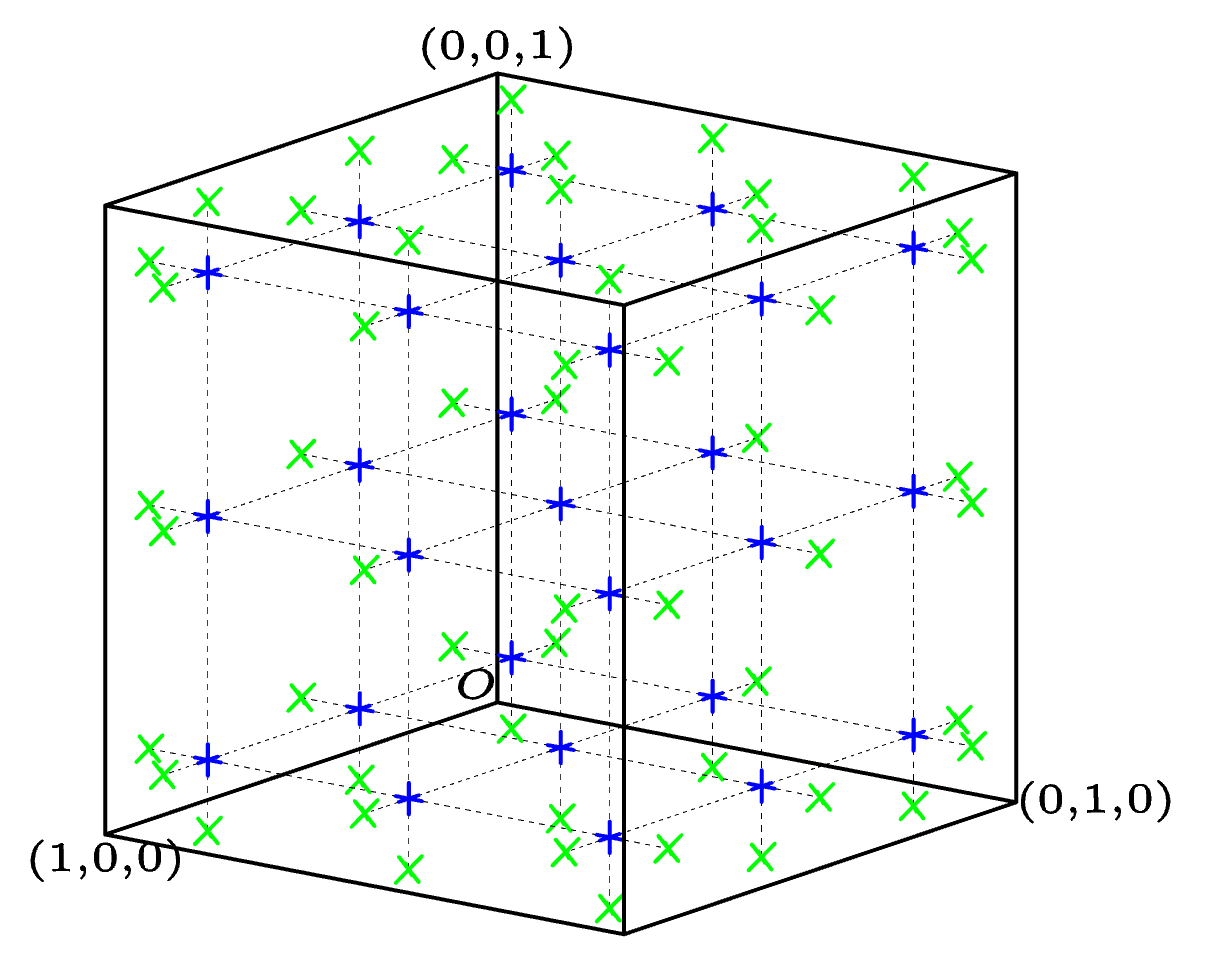
\includegraphics[width=6cm]{ref_element_pg}
  \caption{Volume and face Gauss-Legendre points in the reference
    cube\label{fig:cube-pg}}
\end{figure}

\begin{figure}
  \centering
  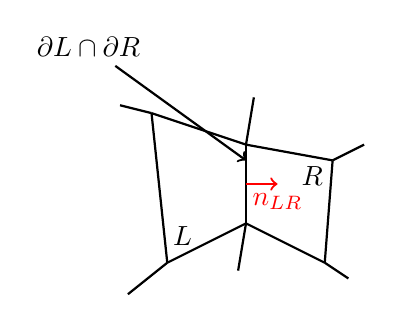
\begin{tikzpicture}[scale=1]
    % intersection
    \draw[thick] (0,1) -- (0,0);
    \draw[->, thick, color=red] (0,0.5) -- (0.4,0.5);
    \node[below, color=red] at (0.4,0.5) {$n_{LR}$};
    \node[above] (n1) at (-2,2) {$\partial L\cap\partial R$};
    \draw[->, thick] (n1) -- (0,0.8);

    % left
    \draw[thick] (-1,-0.5) -- (0,0);
    \draw[thick] (-1.2,1.4) -- (0,1);
    \draw[thick] (-1.2,1.4) -- (-1,-0.5);
    \node[above right] at (-1.05,-0.4) {$L$};

    % right
    \draw[thick] (1,-0.5) -- (0,0);
    \draw[thick] (1.1,0.8) -- (0,1);
    \draw[thick] (1.1,0.8) -- (1,-0.5);
    \node[below left] at (1.1,0.85) {$R$};

    % other quadrangles
    \draw[thick] (0,0) -- (-0.1,-0.6);
    \draw[thick] (0,1) -- (0.1,1.6);
    \draw[thick] (-1,-0.5) -- (-1.5,-0.9);
    \draw[thick] (-1.2,1.4) -- (-1.6,1.5);
    \draw[thick] (1,-0.5) -- (1.3,-0.7);
    \draw[thick] (1.1,0.8) -- (1.5,1);
  \end{tikzpicture}
  \caption{Mesh: notation conventions\label{fig:mesh-conv}}
\end{figure}

%\begin{figure}
%\centering
%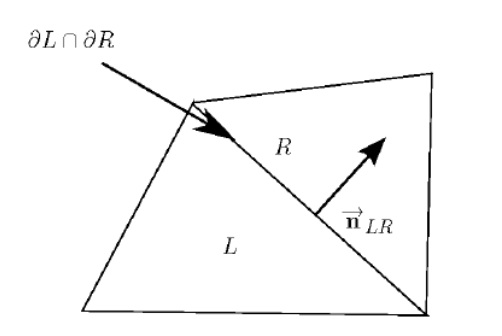
\includegraphics[width=5cm]{cell-LR}
%\caption{Mesh: notation conventions.\label{fig:mesh-conv}}
%\end{figure}
%

\subsubsection{DG Formulation}
The numerical solution satisfies the DG approximation scheme
\begin{eqnarray}
  \forall L,\forall i\quad\int_{L}\partial_{t}\vec{W}\psi_{i}^{L}-\int_{L}\vec{F}(\vec{W},\vec{W},\nabla\psi_{i}^{L}) \nonumber \\
+\int_{\partial L}\vec{F}(\vec{W}_{L},\vec{W}_{R},\vec{n}_{LR})\psi_{i}^{L}=0.
\label{eq:dg}
\end{eqnarray}
In this formula,
\begin{itemize}
\item $R$ denotes the neighbor cells along $\partial L$.
\item $\vec{n}_{LR}$ is the unit normal vector on $\partial L$
  oriented from $L$ to $R$. See Fig.\ref{fig:mesh-conv}.
\item $\vec{F}(\vec{W}_{L},\vec{W}_{R},\vec{n})$ is the numerical
  flux, which satisfies
  $\vec{F}(\vec{W},\vec{W},\vec{n})=F^{k}(\vec{W})\vec{n}_{k}$.
\end{itemize}

Inserting expansion (\ref{eq:expansion}) into (\ref{eq:dg}) we obtain
a system of differential equations satisfied by the
$\vec{W}_{L}^{j}(t)$. This system of differential equations can be
solved numerically with a standard Runge-Kutta method.

The choice of interpolation we have described in the previous section
is well adapted to the DG formulation.  For instance, the nodal basis
property ensures that we have direct access to the values of $\vec{W}$
at the Gauss points. Consequently the mass matrix is diagonal. In
addition, the computation of the volume term $
\int_{L}F(\vec{W},\vec{W},\nabla\psi_{i}^{L})$ it is not necessary to
loop on all the volume Gauss points. Indeed, the gradient of
$\psi_{i}$ is nonzero only at the points that are aligned with point
$i$ (see Fig.\ref{fig:cross}). Finally, for computing the face
integrals \begin{equation}\int_{\partial
    L}F(\vec{W}_{L},\vec{W}_{R},\vec{n}_{LR})\psi_{i}^{L}\end{equation}
we have to extrapolate the values of $\vec{W}$, which are known on the
volume Gauss points, to the interfacial Gauss points. On tetrahedra,
all the volume Gauss points would be involved in the
interpolation. With our nodal hexahedral basis, only the volume Gauss
points aligned with the considered interfacial Gauss point are needed
(see Fig.\ref{fig:cube-pg}: for computing $\vec{W}$ at a green point,
we only need to know $\vec{W}$ at the blue points aligned with this
green point).

In the end, exploiting the tensor basis properties, the DG formulation
(\ref{eq:dg}) in a cell $L$ requires computations of complexity $\sim
D^4$ instead of $\sim D^6$. For high orders, this is a huge
improvement.

\begin{figure}[h]
  \centering
  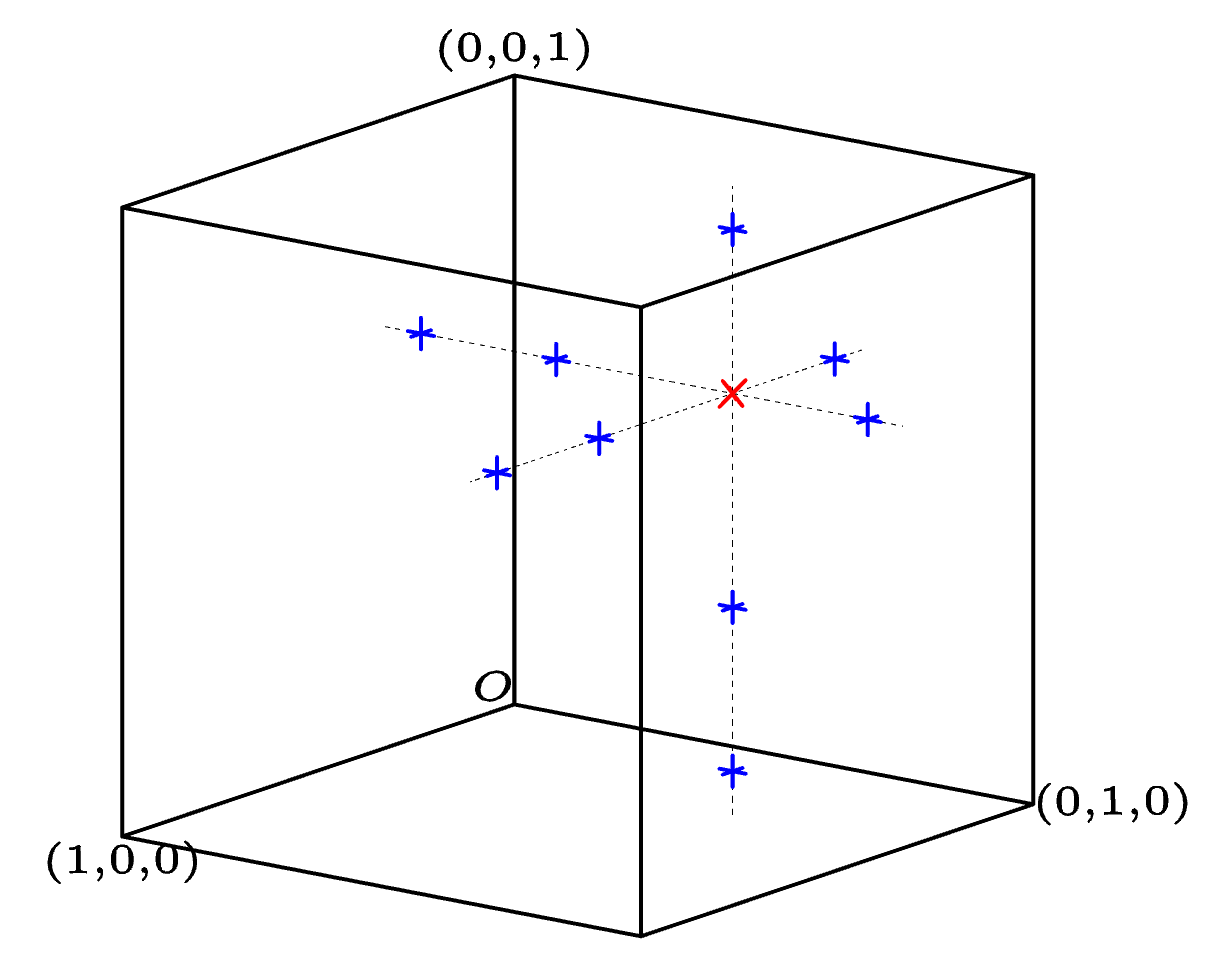
\includegraphics[width=7cm]{ref_element_cross_pg}
  \caption{Non-zero values of the basis functions. The gradient of the
    basis function associated to the red point is nonzero only on the
    blue points}
  \label{fig:cross}
\end{figure}

Beyond these useful optimizations that are also applied in sequential
implementations, The DG method presents many advantages: it is
possible to have different orders on different cells, no conformity is
required between the cell and mesh refinement is thus simplified; the
computations inside a cell only depend on the neighboring cells; the
stencil is more compact than for high order FV methods, so memory
accesses are well adapted to GPU computations; high order inside a
cell implies a high amount of local computations, this property is
well adapted to GPU computations; and finally, two levels of
parallelism can be easily exploited: a coarse grain parallelism, at
the subdomain level, well adapted to MPI algorithms and a fine grain
parallelism, at the level of a single cell, well adapted to OpenCL or
OpenMP.

But there are also possible issues that could make an implementation
inefficient: First, we have first to take care of memory bandwidth,
because unstructured meshes may imply non coalescent memory access.
Moreover, a general DG solver has to manage many different physical
models, boundary conditions, interpolation basis, etc. If the
implementation is not realized with care it is possible to end up with
poorly coded kernels with many barely used variables or branch
tests. Such wastage may remain unseen on standard CPUs with many
registers and large cache memory, but is often catastrophic on GPUs.
Finally, as we have already seen, MPI communications imply very slow
GPU to Host and Host to GPU memory transfers. If possible, it is
advised to hide communication latency by an overlapping with
computations.

\subsection{OpenCL Kernel for a Single GPU}
We first wrote optimized OpenCL kernels for computing, on a single
cell $L$, the terms appearing in the DG formulation (\ref{eq:dg}).
After several experiments, we have found that an efficient strategy is
to write a single kernel for computing the $\partial L$ and $L$
integration steps.

More precisely we construct a kernel with two steps.

In the first step (``flux step''), we compute the fluxes at the faces
Gauss points and store those fluxes in the cache memory of the
work-group. The work-items are distributed on the faces Gauss
points. In this stage, $6(D+1)^2$ work-items are activated.

After a sync barrier, in the second stage (``collecting step''), we
associate a work-item to each volume Gauss point and we collect the
contributions of the other volume Gauss points coming from the
numerical integration. We also collect the contribution from the faces
fluxes stored in the first step. In this stage, $(D+1)^3$ work-items
are activated.

We observe that when the order $D<5$, which is always the case in our
computations, $(D+1)^3 < 6 (D+1)^2$ and then some work-items are
idling in the collecting step.

We have also tried to split the computation into two kernels, one for
the flux step and one for the collecting step, but it requires saving
the fluxes into global memory, and in the end it appears that the
idling work-items method is more efficient.



\subsection{Asynchronous MPI/OpenCL Implementation for Several GPUs}

\subsubsection{Subdomains and Zones}
We have written a generic C++ DG solver called CLAC (``Conservation
Laws Approximation on many Cores'') for solving large problems on
general hexahedral meshes. Practical industrial applications require a
lot of memory and computations. It is thus necessary to address
several accelerators in an efficient way.

We describe some features of the CLAC implementation.

First, the physical models are localized in the code: in practice, the
user has to provide the numerical flux plus a few functions for
applying boundary conditions, source terms, etc. With this approach it
is possible to apply CLAC to very different physics: Maxwell
equations, compressible fluids, MHD, etc. This approach is similar to
the approach of A. Klöckner in \cite{kloeckner2010hedge}.

We also adopt a domain decomposition strategy. The mesh is split into
several domains, each of which is associated to a single MPI node, and
each MPI node is associated to an OpenCL device (CPU or GPU).

In addition to the domain decomposition, in each domain we split the
mesh into zones. We consider volume zones made of hexahedral cells and
also interface zones made of cells faces. The role of a volume zone is
to apply the source terms and the flux balance between cells inside
the zone. The interface zones are devoted to computing the flux
balance between cells of different volume zones. When an interface
zone is at the boundary of the computational domain, it is used for
applying boundary conditions. When it is situated at an interface
between two domains, it is also in charge of the MPI communications
between the domains. Interface zones also serves to manage mesh
refinements between two volume zones. A simple example of mesh with
two subdomains, three volume zones and five interface zones is given
in Fig.\ref{fig:simple-mesh} and a schematic view of the same mesh is
represented in Fig.\ref{fig:scheme-view}. We observe in this figure
that simple non-conformities are allowed between volume zones (for
instance neighboring volume zones 2 and 3 do not have the same
refinement).

Finally, a zone possesses identical elements (same order, same
geometry, same physical model). Thus, different computation kernels
are compiled for each zone, in order to save registers and branch
tests. We have observed that this aspect is very important for
achieving high efficiency. For example, it is possible to simplify the
kernel that compute the flux balance at an interface zone between
two volume zones with conforming meshes. At an interface between
volume zones with different refinements, the kernel is more complex,
because the Gauss integration points are not aligned (see Interface
zone 3 on Fig.\ref{fig:scheme-view}).  The specialized kernels take
advantage of the Gauss points alignment and store interpolation and
geometrical data in constant arrays or preprocessor macros. The
speedup obtained using the specialized kernels as opposed to the
generic kernels is reported in Table \ref{tab:speedup_specialisation}
for different interpolation orders.

\begin{table}[h]
  \centering
  %\caption{A simple non conforming mesh\label{fig:simple-mesh}}
  \caption{Speedup obtained with the specialized kernels}
  \label{tab:speedup_specialisation}
  \begin{tabular}[h]{|c||c|c|c|c|c|}
    \hline
    Order   &   0 &   1 &   2 &   3 &   4 \\ \hline
    Speedup & 1.6 & 1.8 & 2.8 & 3.6 & 5.5 \\ \hline
  \end{tabular}
\end{table}

\begin{figure}
  \centering
  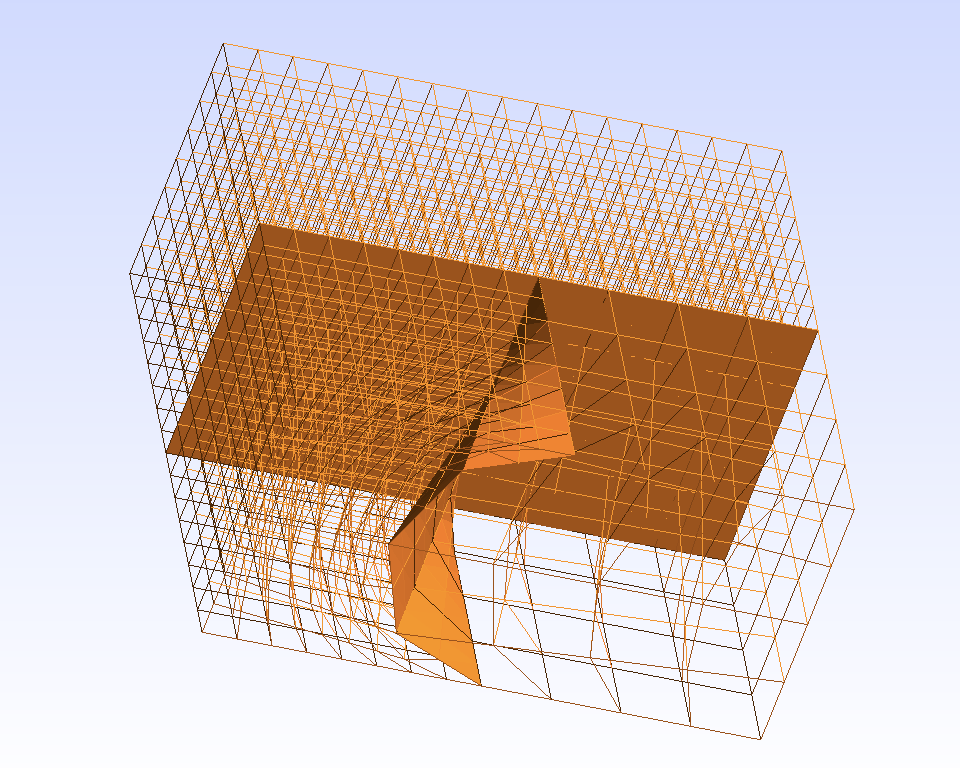
\includegraphics[width=6cm]{3zones-gmsh}
  \caption{A simple non conforming mesh\label{fig:simple-mesh}}
\end{figure}


\begin{figure}
  \centering
  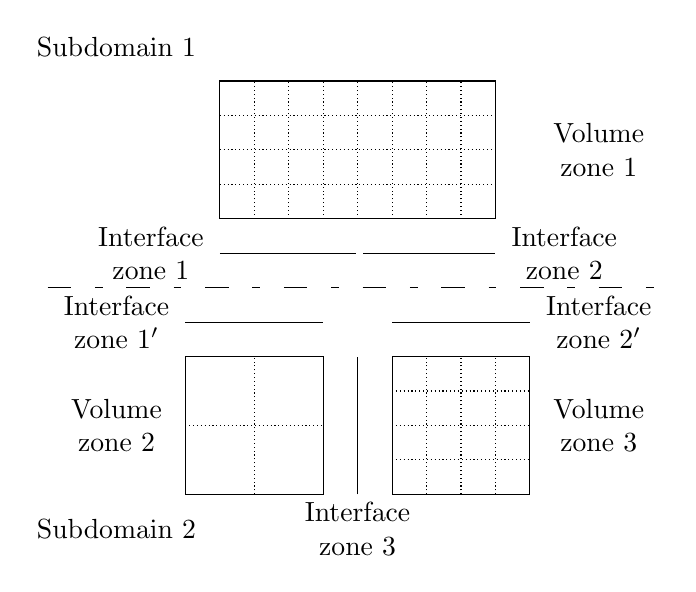
\begin{tikzpicture}[scale=1.75]
    \draw[densely dotted] (0,0) grid[step=0.5] (1,1);
    \draw (0,0) rectangle (1,1);

    \draw[densely dotted] (1.5,0) grid[step=0.25] (2.5,1);
    \draw (1.5,0) rectangle (2.5,1);

    \draw[densely dotted] (0.25,2) grid[step=0.25] (2.25,3);
    \draw (0.25,2) rectangle (2.25,3);

    \draw[dash pattern=on 3mm off 3mm on 1mm off 3mm] (-1,1.5) --(3.5,1.5);
    \draw (1.25,0) -- (1.25,1);
    \draw (0,1.25) -- (1,1.25);
    \draw (1.5,1.25) -- (2.5,1.25);
    \draw (0.25,1.75) -- (1.24,1.75);
    \draw (1.29,1.75) -- (2.25,1.75);

    \node at (-0.5,3.25) {Subdomain 1};
    \node at (-0.5,-0.25) {Subdomain 2};

    \node[align=center] at (3,2.5) {Volume\\zone 1};
    \node[align=center] at (-0.5,0.5) {Volume\\zone 2};
    \node[align=center] at (3,0.5) {Volume\\zone 3};

    \node[align=center] at (-0.5,1.25) {Interface\\zone $1'$};
    \node[align=center] at (3,1.25) {Interface\\zone $2'$};
    \node[align=center] at (1.25,-0.25) {Interface\\zone 3};
    \node[align=center] at (-0.25,1.75) {Interface\\zone 1};
    \node[align=center] at (2.75,1.75) {Interface\\zone 2};

  \end{tikzpicture}
  \caption{Schematic view of the simple mesh\label{fig:scheme-view}}
\end{figure}


%\begin{figure}
%  \centering
%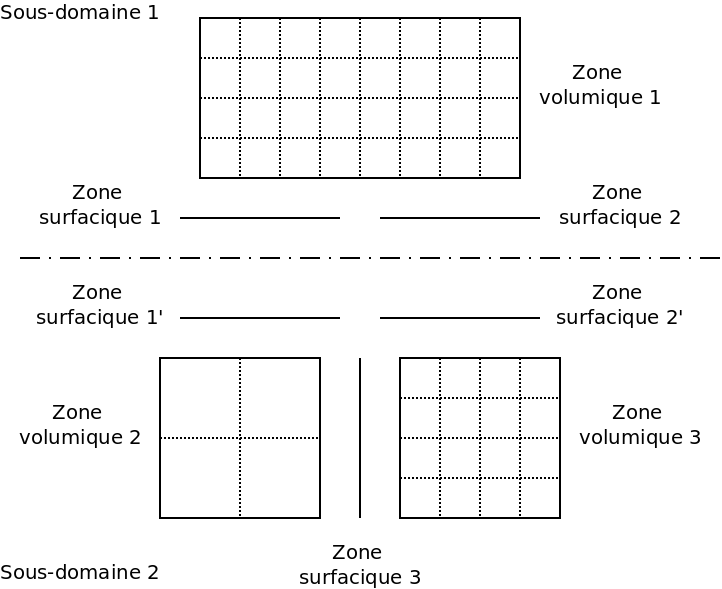
\includegraphics[width=6cm]{schema_exemple}
%\caption{Schematic view of the siumple mesh.\label{fig:scheme-view}}
%\end{figure}
%
%\begin{figure*}
%  \centering
% 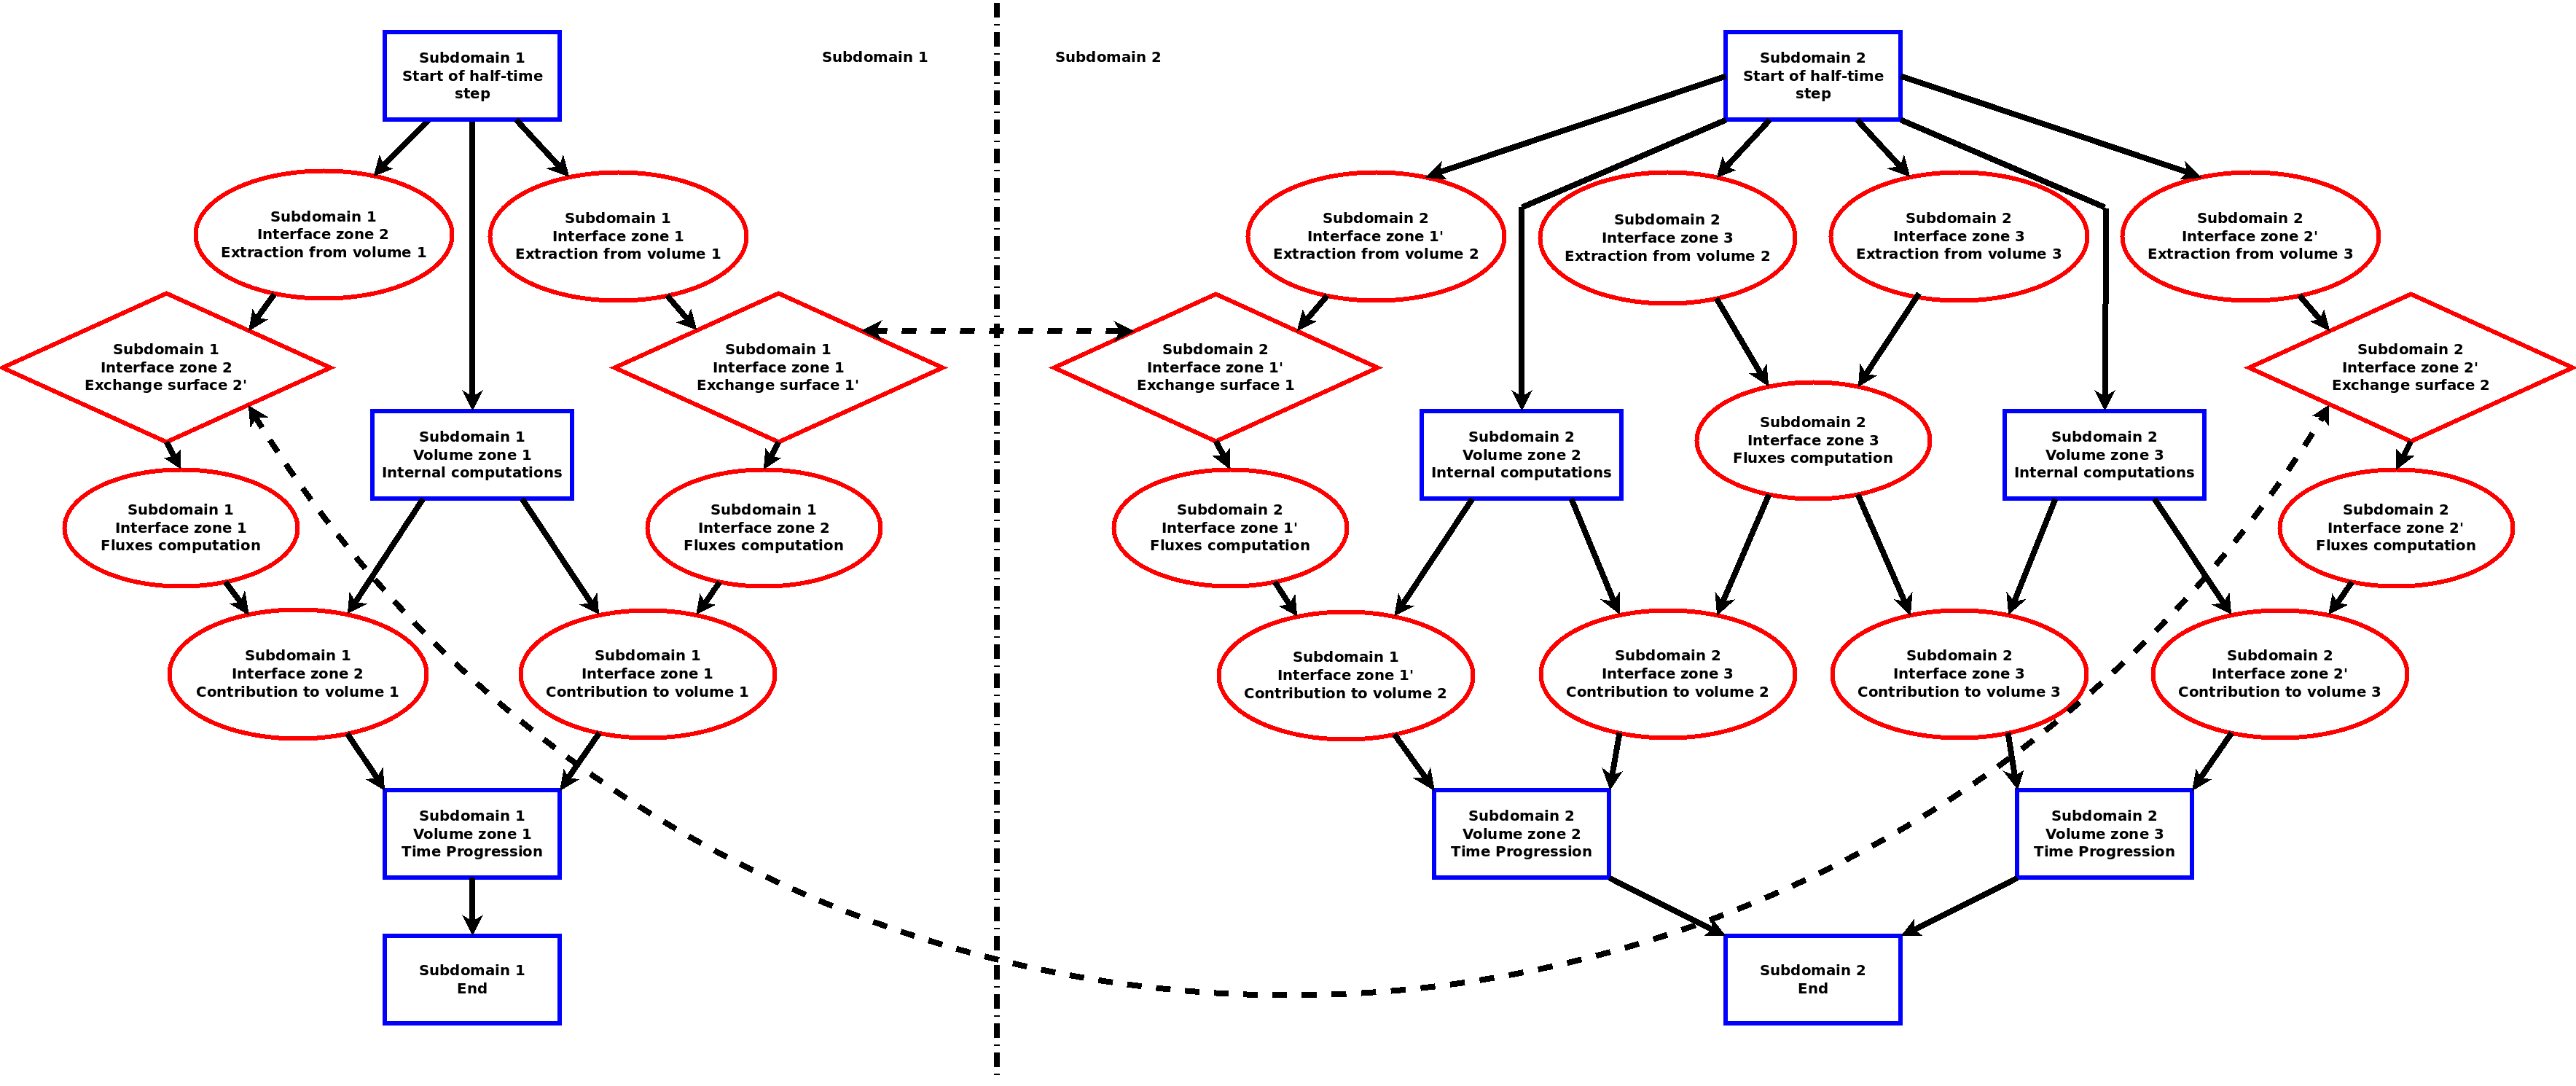
\includegraphics[width=17cm]{graph_exemple}
%  \caption{Task graphs for the simple mesh. One task graph for each MPI node.}
%  \label{fig:mpi-task-graph}
%\end{figure*}

\begin{figure*}
  \centering
  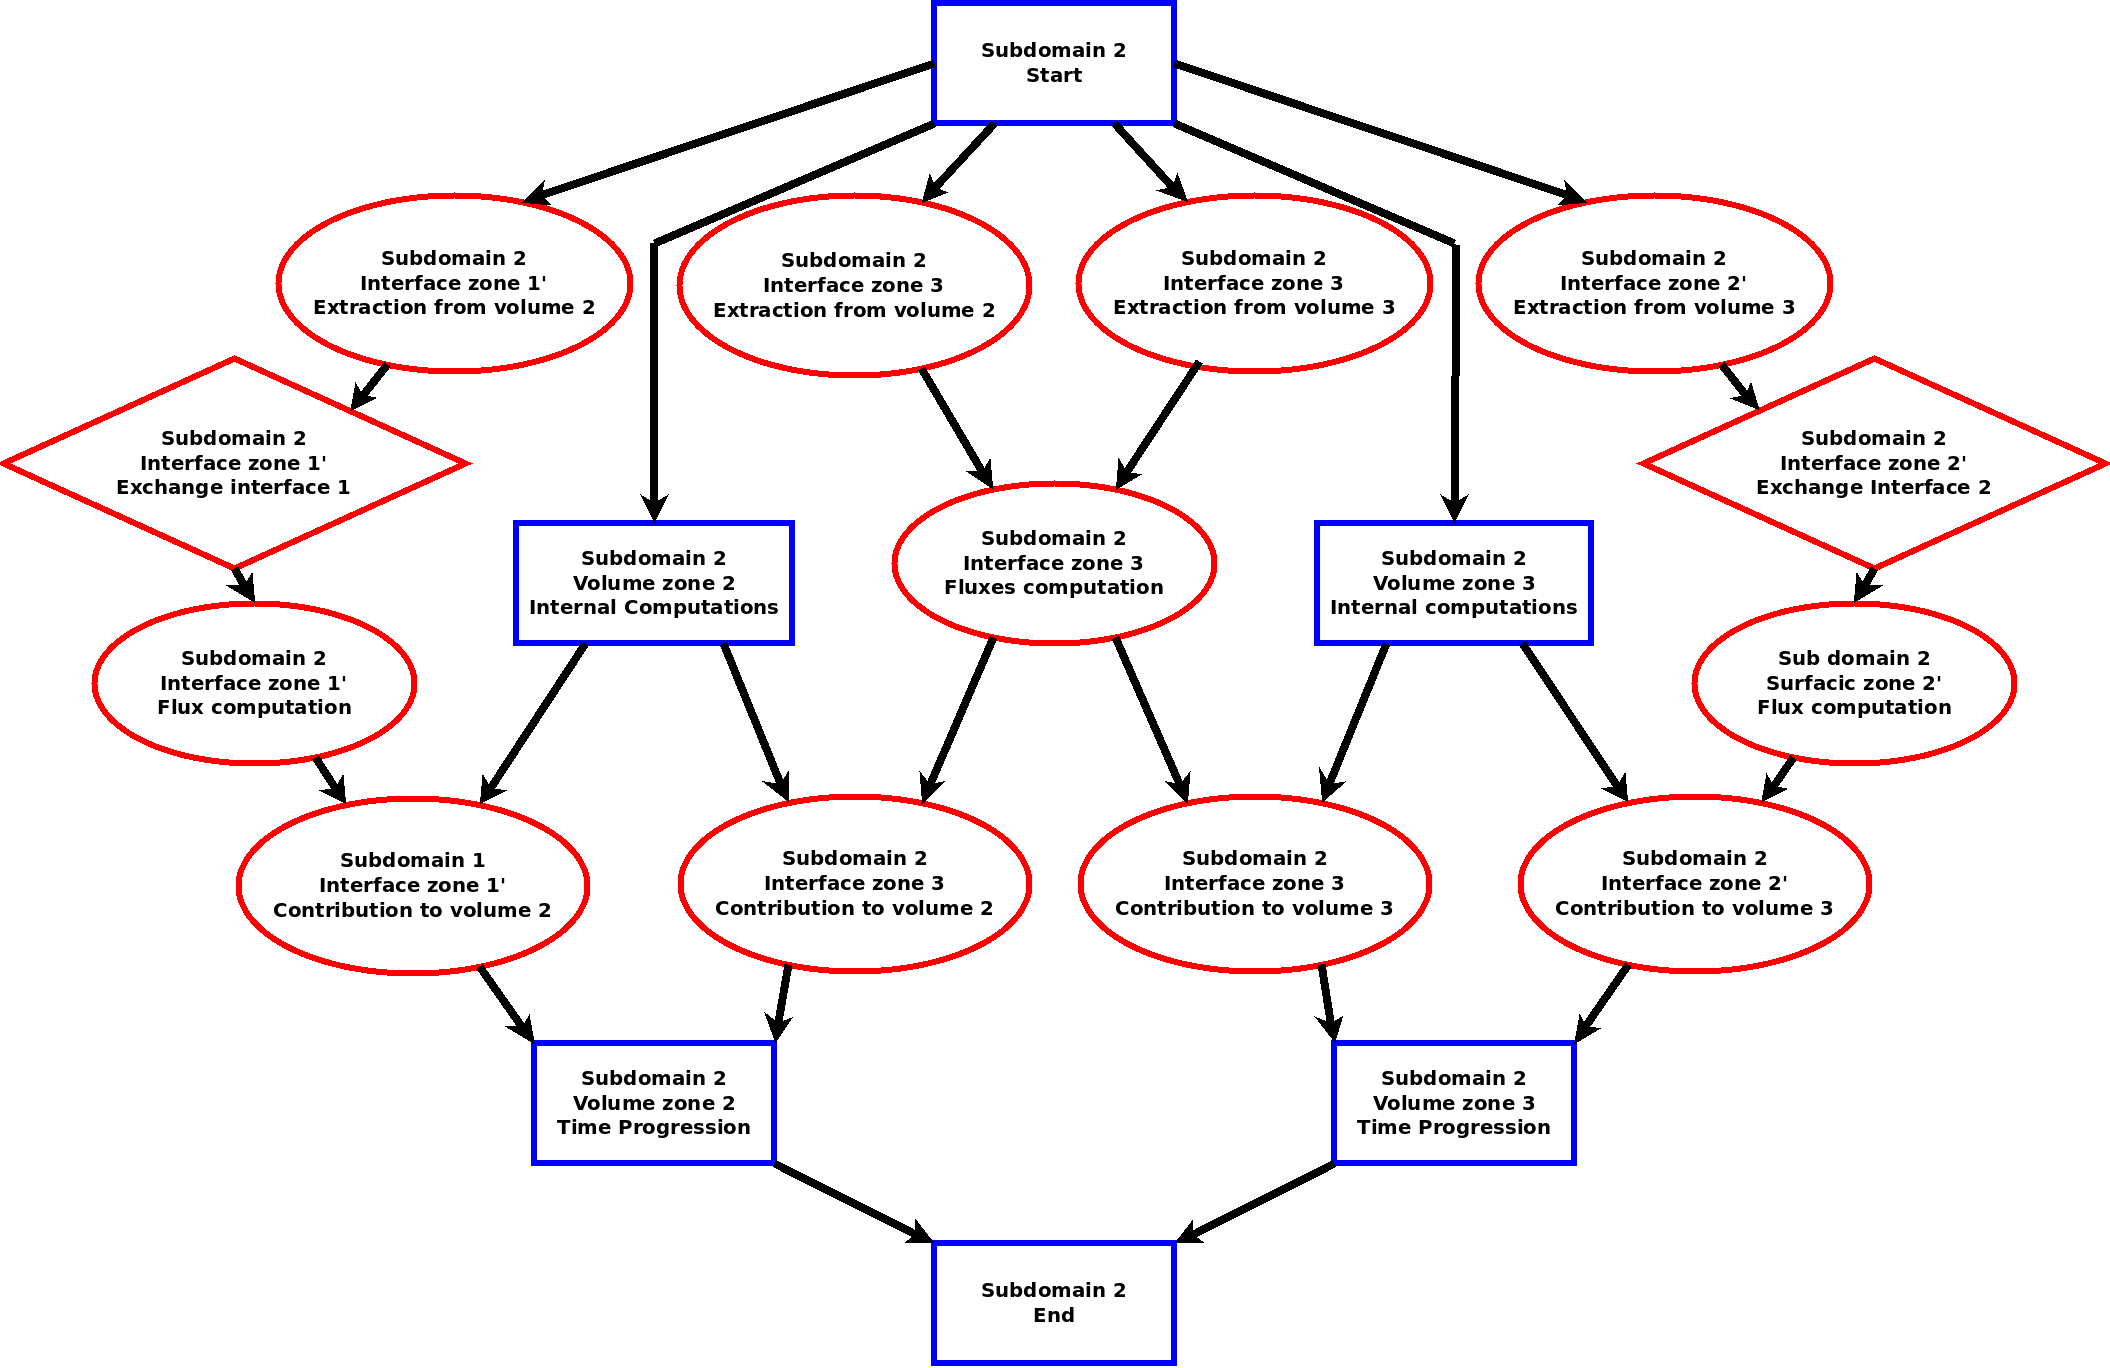
\includegraphics[width=10cm]{graph_exemple_2}
  \caption{Task graph for subdomain 2}
  \label{fig:sub2-task-graph}
\end{figure*}


\subsubsection{Task Graph}
The zone approach is very useful to express the dependency between the
different tasks of the DG algorithm.

We have identified tasks attached to volume or interface zones that
have to be executed for performing a Runge-Kutta substep with the DG
formulation. Those tasks are detailed in Table \ref{tab:tasks}.

\begin{table}[h]
  \centering
  \caption{Tasks description}
  \label{tab:tasks}
  \begin{tabular}{|c|c|m{4cm}|}
    \hline
    Name & Attached to & Description\tabularnewline
    \hline
    \hline
    Extraction & Interface & Copy or extrapolate the values of $W$ from a neighboring volume
    zone \tabularnewline
    \hline
    Exchange & Interface & GPU/Host transfers and MPI communication with an interface of another domain\tabularnewline
    \hline
    Fluxes & Interface & Compute the fluxes at the Gauss points of the interface\tabularnewline
    \hline
    Sources & Volume & Compute the internal fluxes and source terms inside a volume zone\tabularnewline
    \hline
    Boundaries & Interface & Apply the fluxes of an interface to a volume zone\tabularnewline
    \hline
    Time & Volume & Apply a step of the Runge-Kutta time integration to a volume zone\tabularnewline
    \hline
    Start & Volume & Fictitious task: beginning of the Runge-Kutta substep\tabularnewline
    \hline
    End & Volume & Fictitious task: end of the Runge-Kutta substep\tabularnewline
    \hline
  \end{tabular}
\end{table}

We express the dependencies between the tasks in a graph, and
construct a task graph per subdomain. For instance, we have
represented on Fig.\ref{fig:sub2-task-graph} the task graph associated
to Subdomain 2 of the simple mesh of Fig.\ref{fig:scheme-view}. The
volume tasks are represented in blue rectangles, the interface tasks
in red ellipses. The interface tasks that require MPI communication
are in red rhombuses.

We observe in these figures that it is possible to perform the
exchange tasks and the internal computations at the same time. It is
thus possible to overlap communications and GPU/Host transfers by
computations.

OpenCL contains events objects for describing task dependencies
between the operations sent to command queues. It is also possible to
create user events for describing interactions between the OpenCL
command queues and tasks that are executed outside of a call to the
OpenCL library. We have decided to rely only on the OpenCL event
management for constructing the task dependencies.

Using asynchronous MPI communication requires calling
\texttt{MPI\_Wait} before launching tasks that depend on the
completion of communication. We thus face a practical problem, which
is to express the dependency between MPI and OpenCL operations in a
non-blocking way. A possibility would have been to use an OpenCL
``Native Kernel'' containing MPI calls. A native kernel is a standard
function compiled and executed on the host side, but that can be
inserted into the OpenCL task graph. As of today, the native kernel
feature is not implemented properly in all the OpenCL drivers. We thus
had to adopt another approach in order to circumvent this difficulty.

Our solution uses the C++ standard thread class. It is also necessary
to use an MPI implementation that provides the
\texttt{MPI\_THREAD\_MULTIPLE} option.  For programming the
``Exchange'' task, we first create an OpenCL user event.  Then we
launch a thread and return from the task.  The main program flow is
not interrupted and other operations can be enqueued. Meanwhile, in
the thread, we start a blocking send/recv MPI operation for exchanging
data between the boundary interface zones.  Because the communication
is launched in a thread, its blocking or non-blocking nature is not
very important.  When the communication is finished, we mark the
OpenCL event as completed and exit the thread.  The completion of the
user event triggers the beginning of the enqueued tasks that depend on
the exchange.

As we will see in the next section, this simple solution offers very
good efficiency.

\subsection{Efficiency Analysis}
In this section we measure the efficiency of the CLAC
implementation. Recently the so-called roofline model has been
introduced for analyzing the efficiency of algorithm implementation on
a single accelerator \cite{williams2009roofline}. This model is based
on several hardware parameters.  First, we need to know the peak
computation performances of the accelerator. This peak is measured
with an algorithm with high computational intensity and very little
memory access. It can be measured with a program that only requires
register access. For instance, for a NVIDIA K20 accelerator, the peak
performance is $P=3.5\hbox{TFLOP/s}.$ Another parameter is the memory
bandwidth $B$ that measures the transfer speed of the global
memory. For a NVIDIA K20 $B=208\hbox{GB/s}.$


Not all algorithms are well adapted to GPU computing. Consider an
algorithm (A) in which we count $N_{\hbox{ops}}$ operations (add,
multiply, etc.) and $N_{\hbox{mem}}$ global memory operations (read or
write). In \cite{williams2009roofline}, the computational intensity of
the algorithm is defined by
\begin{equation}I=\frac{N_{\hbox{ops}}}{N_{\hbox{mem}}}.\end{equation}
The maximal attainable performance of one GPU for this algorithm is then given by the roofline formula:
\[
P_{A}=\max(P,B\times I).
\]

We have counted the computational and memory operations of our DG
implementation. The counting method is simply based on source
inspection because we have not been able to find an automatic and
reliable tool for evaluating the amount of floating point and memory
operations. We only count memory transfer to the global memory,
floating point and integer operations: we neglected pointer
arithmetic and register accesses.  The results are plotted in
Fig.\ref{fig:roofline}. We observe that for order 1, the DG method is
limited by the memory bandwidth.  For higher orders, the method is
limited by the peak performance of the GPU. The figure confirms that
the DG method is well adapted to GPU architectures.  We have also
performed this analysis for the FV method described in Sect.2. For
large grids, the efficiency of the FV scheme is approximately $20$
FLOP/B. The FV algorithm is thus also limited by the peak performance
of the GPU. Our implementation of the FV scheme reaches approximately
$800$ GFLOP/s on a single K20 GPU.

\begin{figure}[h]
  \centering
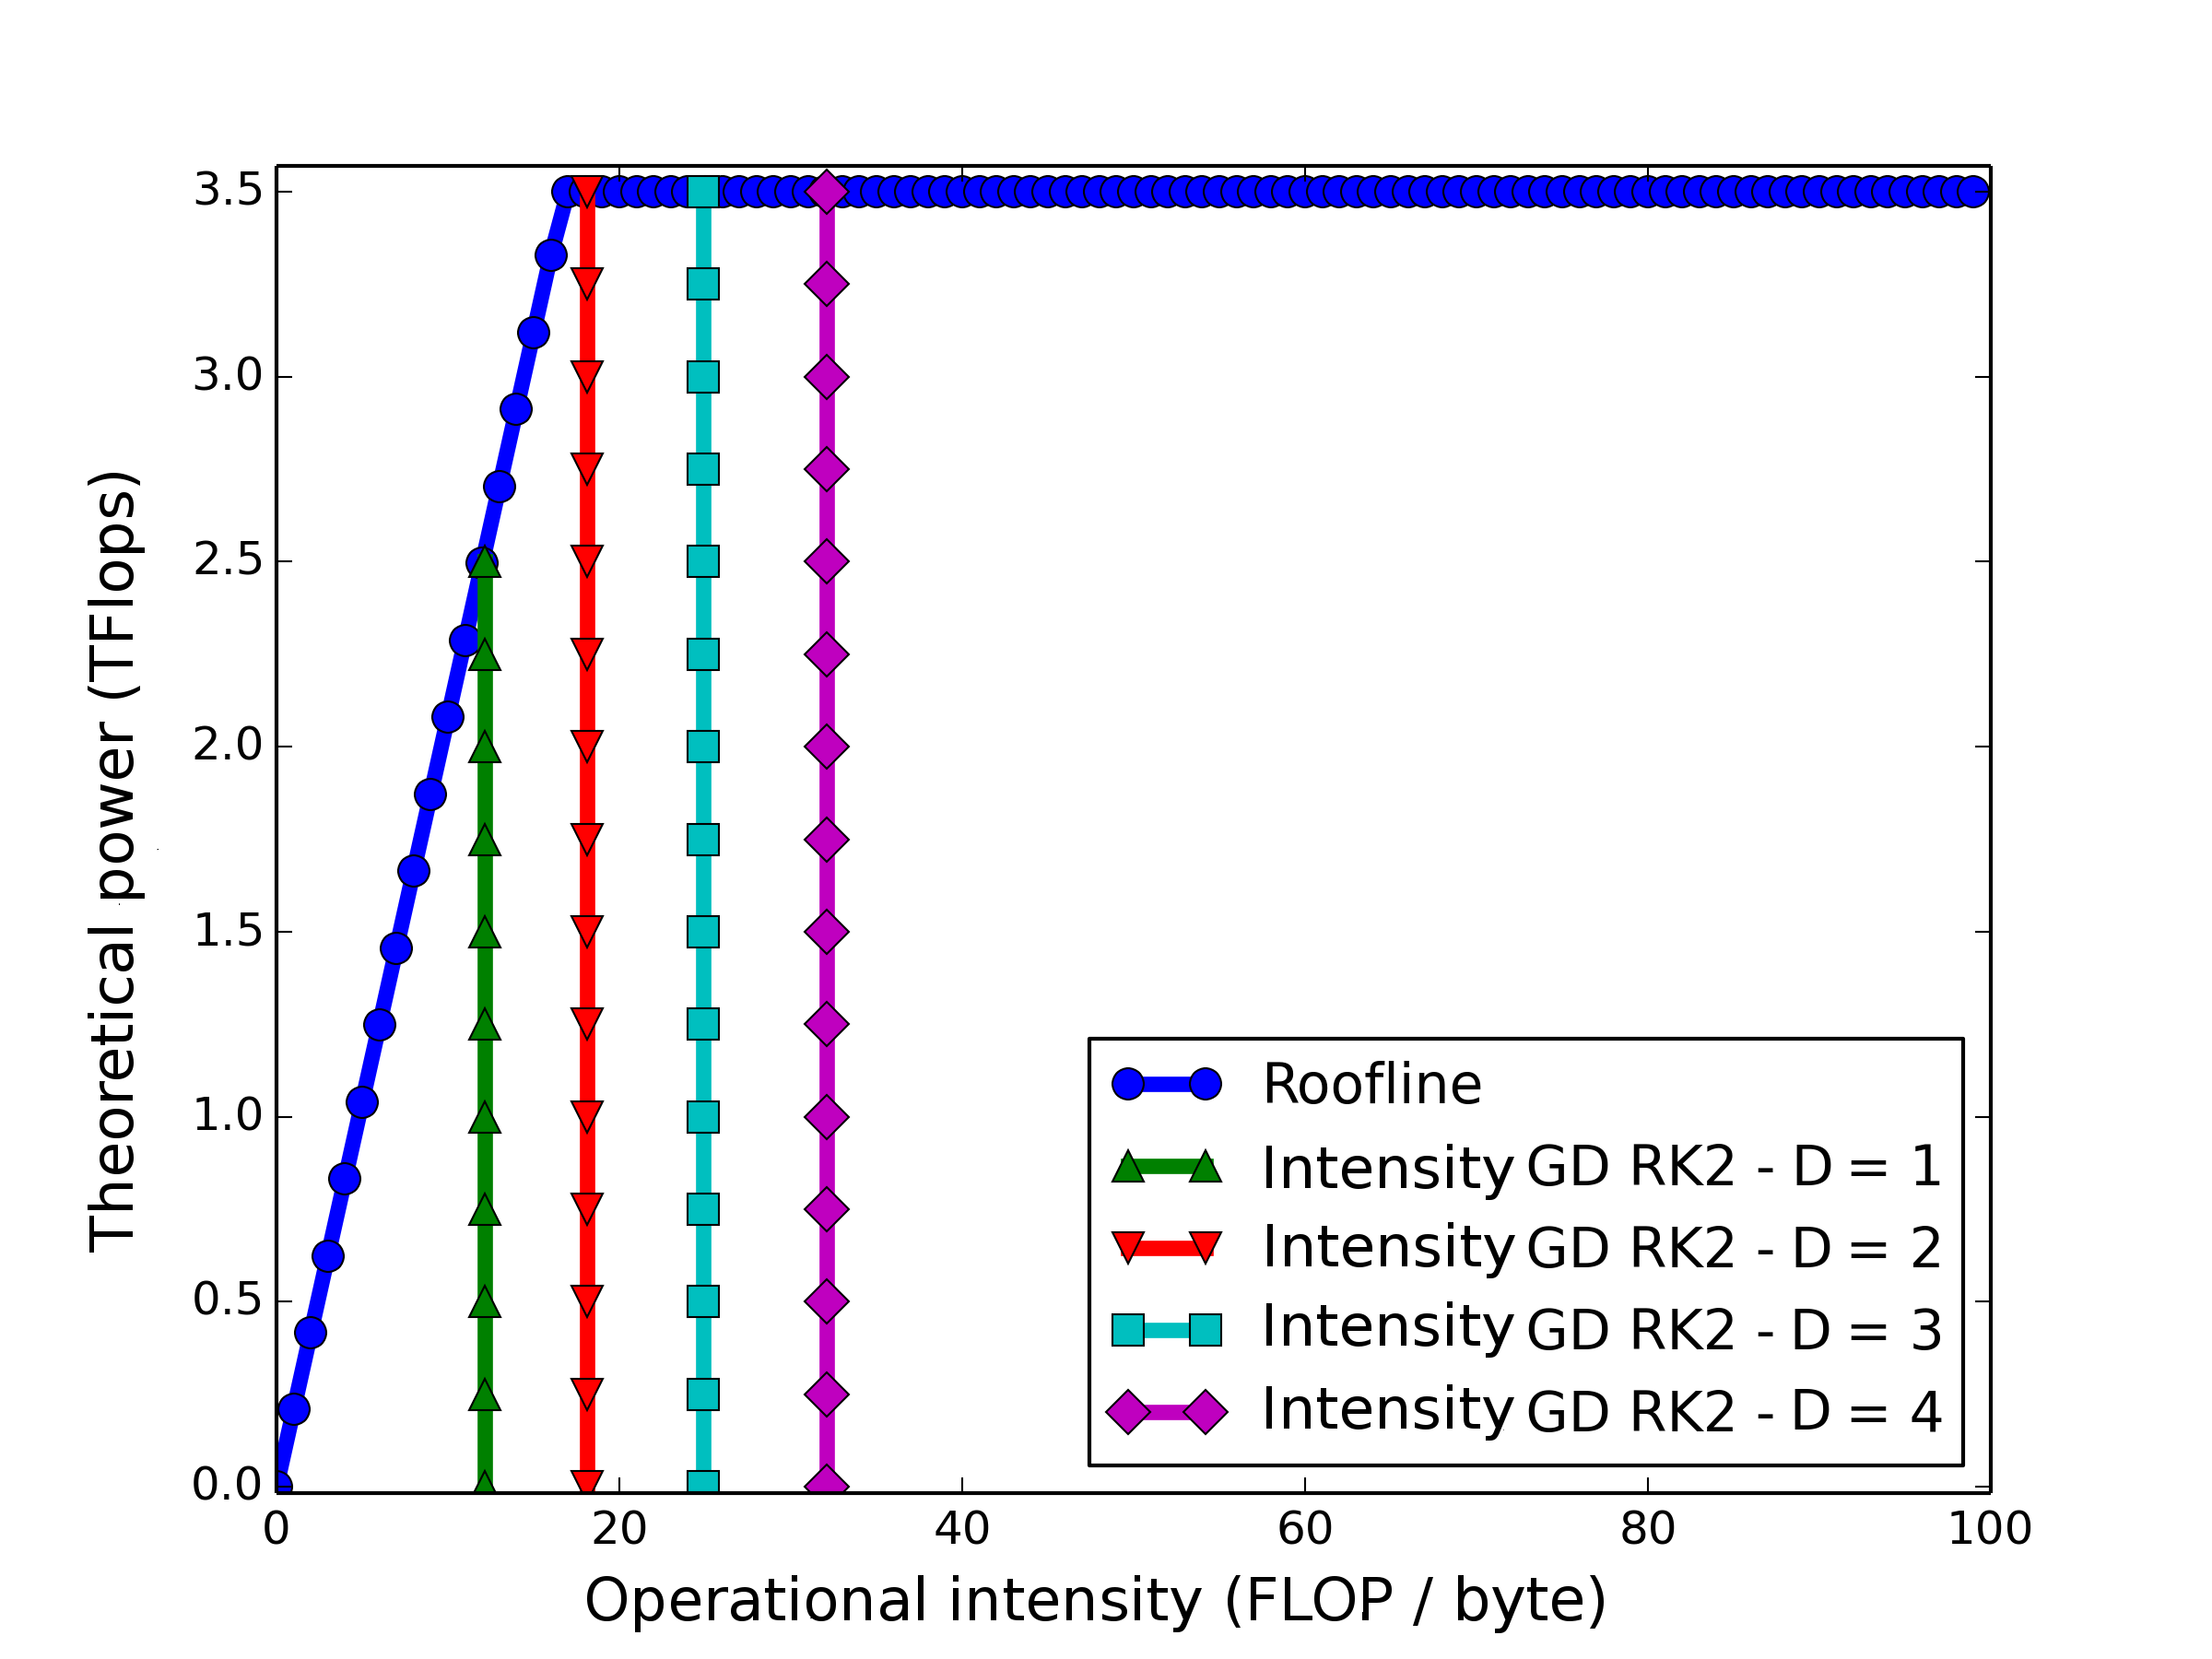
\includegraphics[width=7cm]{roof_line_clac2}
  \caption{Roofline model and DG method. Abscissa: computational
    intensity $I$ (FLOP/B). Ordinate: Algorithm performance
    (TFLOP/s) \label{fig:roofline}}
\end{figure}

In Table \ref{tab:async-perfs}, we present the results that we have
measured with the asynchronous MPI/OpenCL implementation with 1, 2, 4
and 8 GPUs. For comparison, we also give in Table \ref{tab:sync-perfs}
the results of the synchronous execution (we wait that each task is
completed before launching the next one). The computational domain
$\Omega$ is a cube. The chosen model is the Maxwell system
($m=6$). The mesh is made of several subdomains of $90^3$ cells. We
perform single precision computations. The interpolation is of order
$D=3$. The algorithm requires storing three time steps of the
numerical solution. With these parameters the memory of each K20 board
is almost entirely filled. Indeed the storage of the electromagnetic
field on one subdomain requires approximately $3.4$ GB.

\begin{table}[htp]
  \begin{center}
    \caption{Weak scaling of the synchronous MPI/OpenCL
      implementation \label{tab:sync-perfs}}
    \begin{tabular}{|c|c|c|c|c|}
      \hline
      & 1 GPU & 2 GPUs & 4 GPUs & 8 GPUs\tabularnewline
      \hline
      \hline
      TFLOP/s & 1.01 & 1.84 & 3.53 & 5.07\tabularnewline
      \hline
      Speedup & 1 & 1.83 & 3.53 & 5.01\tabularnewline
      \hline
    \end{tabular}
  \end{center}
\end{table}%

\begin{table}[htp]
  \begin{center}
    \caption{Weak scaling of the asynchronous MPI/OpenCL implementation \label{tab:async-perfs}}
    \begin{tabular}{|c|c|c|c|c|}
      \hline
      & 1 GPU & 2 GPUs & 4 GPUs & 8 GPUs\tabularnewline
      \hline
      \hline
      TFLOP/s & 1.01 & 1.96 & 3.78 & 7.34\tabularnewline
      \hline
      Speedup & 1 & 1.94 & 3.74 & 7.26\tabularnewline
      \hline
    \end{tabular}
  \end{center}
\end{table}%


We observe in Table \ref{tab:async-perfs} that the asynchronous
implementation is rather efficient and that the communications are
well overlapped by the GPU computations. In addition, we observe that
with CLAC we attain approximately $30\%$ of the roofline limit. This
result is not too bad, because CLAC handles unstructured meshes and
some non-coalescent memory access are unavoidable.


\subsection{Numerical Results}


For finishing this paper, we would like to present numerical results
that we have obtained from a real-world application. The objective is
to compute the reflection of an electromagnetic plane wave with
Gaussian profile over an entire aircraft. The mesh is made of
$3,337,875$ hexahedrons. We used an order $D=2$ approximation and 8
GPUs (NVIDIA K20). The interior and the exterior of the aircraft are
meshed. In order to approximate the infinite exterior model, we use a
Perfectly Matched Layers (PML) model~\cite{berenger}. The PML model is
an extension of the Maxwell model. The possibility to use different
models in different zones is here exploited for applying the PML
model. In a PML zone, the Maxwell equations are coupled with a system
of six ordinary differential equations. This coupling induces an
additional cost reported in Table \ref{tab:cost_pml}.


\begin{table}[h]
  \centering
  \caption{Additional cost for 5 and 10 PML expressed in percentage of the
    total computation time}
  \label{tab:cost_pml}
  \begin{tabular}[h]{|c||c|c|c|c|c|}
    \hline
             Order &    0 &    1 &    2 &    3 &    4 \\ \hline
     5 layers (\%) & 7.14 & 4.29 & 15.9 & 16.5 & 15.0 \\ \hline
    10 layers (\%) & 7.95 & 6.49 & 19.0 & 20.6 & 18.1 \\ \hline
  \end{tabular}
\end{table}

%The current density on the aircraft is given in Fig.\ref{fig:current} at a chosen time.
%
%\begin{figure}[h]
%\begin{center}
%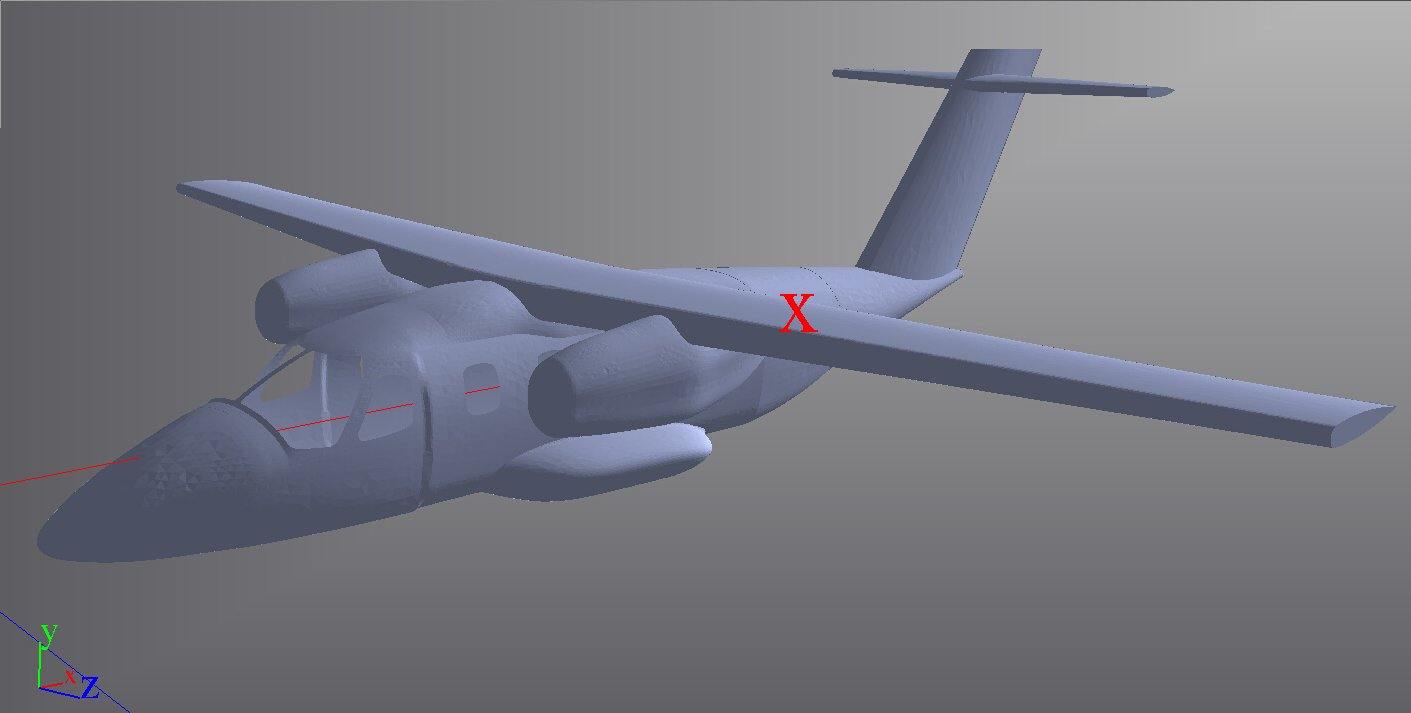
\includegraphics[width=7cm]{ntc1-unstructured}
%\par\end{center}
%\caption{Aircraft. Only the mesh skin is represented.\label{fig:ntc1}}
%\end{figure}
%
%
%
%\begin{figure}[h]
%\begin{center}
%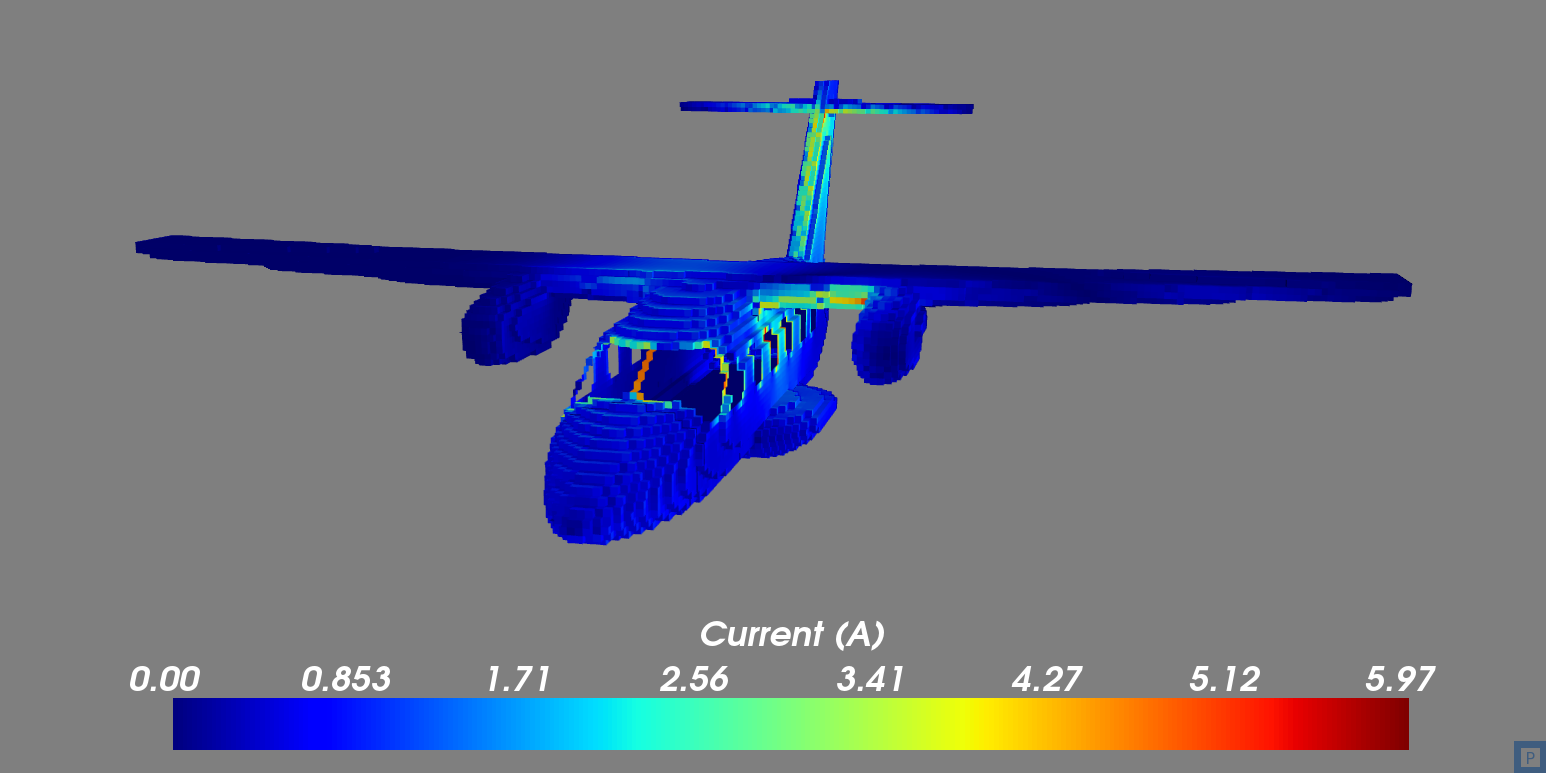
\includegraphics[width=8cm]{current}
%\par\end{center}
%\caption{Current density on the aircraft skin.\label{fig:current}}
%\end{figure}
%


\section{Conclusions}
In this work we have reviewed several methods for solving hyperbolic
conservation laws. Such models are very useful in many fields of
physics or engineering.  We have presented a finite volume OpenCL/MPI
implementation. We have seen that coalescent memory access is
essential for obtaining good efficiency. The synchronous MPI
communication does not allow an optimal scaling with several
GPUs. However the MPI extension allows addressing computations that
would not fit into a single accelerator.

We have then presented a more sophisticated approach: the
Discontinuous Galerkin method on unstructured hexahedral meshes. We
have also written an OpenCL/MPI implementation of the method. Despite
the unstructured mesh and some non-coalescent memory accesses, we
reach 30\% of the peak performance.

In future works we intend to change the description of the mesh
geometry in order to minimize the memory access: we can for instance
share a higher order geometrical transformation $\tau$ between several
cells. We also plan to implement a local-time stepping algorithm in
order to be able to deal with locally refined meshes.  Finally, we
would like to describe the task graph in a more abstract manner in
order to distribute the computation more effectively on the available
resources. An interesting tool for performing such distribution could
be for instance the StarPU environment~\cite{augonnet2011starpu}.


%ACKNOWLEDGMENTS are optional
\section{Acknowledgments}
This work has benefited from several supports: from the French Defense
Agency DGA, from the Labex ANR-11-LABX-0055-IRMIA and from the AxesSim
company.  We also thank Vincent Loechner for his helpful advice
regarding the optimization of the OpenMP code.

%
% The following two commands are all you need in the
% initial runs of your .tex file to
% produce the bibliography for the citations in your paper.
\bibliographystyle{abbrv}
%\nocite{*}
\bibliography{helluy-sppexa-2016}  % sigproc.bib is the name of the Bibliography in this case
% You must have a proper ".bib" file
%  and remember to run:
% latex bibtex latex latex
% to resolve all references
%
% ACM needs 'a single self-contained file'!
%
%APPENDICES are optional
%\balancecolumns
%\appendix
%Appendix A
\end{document}

%%  LocalWords:  IWOCL OpenCL MPI Helluy Université de Inria TONUS FV
%%  LocalWords:  Strub AxesSim Sapidus Illkirch Massaro Galerkin DG
%%  LocalWords:  OpenMP GPU PDE hyperbolicity Jacobian diagonalizable
%%  LocalWords:  multiphase MHD Vlasov plasmas Euler's polytropic RL
%%  LocalWords:  subdomain optimizations multicore prefetching Strang
%%  LocalWords:  piecewise  centers gcc unoptimized subgrids supremum
%%  LocalWords:  parallelize subgrid SMP SIMD GPUs CPUs neighboring
%%  LocalWords:  PCIe runtime AMD NVIDIA subdomains recv neighbor HD
%%  LocalWords:  OpenGL interops scalability color gray center det
%%  LocalWords:  hexahedral tetrahedra hexahedra cccccccc Runge Kutta
%%  LocalWords:  CLAC Klöckner conformities substep enqueued roofline
%%  LocalWords:  perfs TFLOP mem hexahedrons PML Starpu defense DGA
%%  LocalWords:  Acknowledgments Labex ANR LABX IRMIA helluy iwocl
%%  LocalWords:  interfacial prefetch Xeon Radeon NVidia preprocessor

%%  LocalWords:  Tonus Friedrichs CUDA hyperthreading Lobatto GFLOP
%%  LocalWords:  StarPU Loechner sppexa
